% Großer Beleg in deutsch.
\documentclass[gb,ngerman]{stthesis}

% Nur Titelseite in TUD-Layout, Rest in SWT-Layout
\usepackage[titlepageonly]{tudlayout}
\usepackage{longtable}
\usepackage{tabu}
\usepackage{multirow}
\usepackage{mathtools}
\usepackage{wasysym}
\usepackage{listings}

% Titel
\title{Migration der SoftAudit-Metriken \newline nach SonarQube}
% Author
\author{Jan Rucks}
% Datum Abgabedatum
\date{09.02.2017}
% Geburtstag
\birthday{07.11.1987}
% Geburtsort
\birthplace{Jena}
% Betreuer
\supervisor{Dr.-Ing. Birgit Demuth}

\hyphenation{Interpretations-spielraum}
\bibliographystyle{alpha}
\lstset{language=java}

\begin{document}
	\maketitle 
	\chapter*{Aufgabenstellung}
		SoftAudit ist ein Werkzeug, um den Zustand eines bestehenden Softwaresystems auf Basis einer statischen Programmanalyse zu ermitteln. Zum einen wird es zur Qualitätssicherung einer Software und zum anderen zur Bewertung einer Software eingesetzt. Die Qualitätssicherung erfolgt durch eine Prüfung der Software hinsichtlich Verletzung von Codierungsregeln und liefert Mängelberichte. Eine Bewertung der Software wird durch die Messung von Quantitäts-, Komplexitäts- und Qualitäts-Metriken durchgeführt. Das Tool SoftAudit wurde von Harry Sneed entwickelt und unterstützt die Programmanalyse für verschiedene Programmiersprachen. SoftAudit wurde bis einschließlich des Wintersemesters 2014/15 im Softwarepraktikum des Lehrstuhls Softwaretechnologie zur Bewertung der Codequalität der studentischen Praktikumsprojekte am Ende der Projektlaufzeit eingesetzt. Allerdings läuft das Tool noch in einer DOS-Umgebung und liefert die Metrik-Berichte in Form einer proprietären Textdatei. \newline
		SonarQube ist eine Plattform ebenfalls für die statische Programmanalyse und analysiert den Code hinsichtlich verschiedener Qualitätseigenschaften. Die Ergebnisse werden in einer Webseite dargestellt. Die SonarQube-Plattform ist modular und erweiterbar aufgebaut. SonarQube ermöglicht über einen Plugin-Mechanismus Erweiterungen in SonarQube zu integrieren. Im Softwarepraktikum am Lehrstuhl Softwaretechnologie wurde SonarQube im WS 2015/16 erstmals zur Bewertung der studentischen Praktikumsprojekte als Teil des Continuous Integration-Prozesses eingesetzt und erlaubt damit auch eine kontinuierliche Bewertung des Projektfortschritts während der Bearbeitungszeit. \newline
		Aufgabe des großen Beleges ist es die aussagekräftigen Komplexitäts- und Qualitäts-Metriken des SoftAudit-Tools nach SonarQube zu migrieren. Dazu soll der Plugin-Mechanismus von SonarQube benutzt werden. \newline
		
		Es sollen folgende Teilaufgaben gelöst werden: 
		\begin{itemize}
		\item Einarbeitung in die Tools SoftAudit und SonarQube
		\item Darstellung der Komplexitäts- und Qualitäts-Metriken nach SNEED
		\item Literaturanalyse zu verwandten Arbeiten
		\item Analyse, welche der SoftAudit-Metriken (Quantität, Komplexität und Qualität) in SonarQube bereits unterstützt werden
		\item Ermittlung der Anforderungen an die Erweiterung von SonarQube um die nicht unterstützten SoftAudit-Metriken
		\item Entwurf und Implementierung der Erweiterungen von SonarQube unter Nutzung des Plugin-Mechanismus von SonarQube für die Programmiersprache Java
		\item Konfiguration von SonarQube für das Softwarepraktikum
		\item Erprobung der Lösung anhand von studentischen Softwareprojekten
		\item Bewertung der Lösung
		\end{itemize}
		
	\tableofcontents
  
	\chapter{Einleitung}
  		Die vorliegende Arbeit gliedert sich in das weite Forschungsfeld der Softwarevermessung ein. Neben dem hier verfolgten Ziel die in studentischen Praktikumsprojekten entstandene Software zu bewerten kann dies in der Praxis aus verschiedensten Gründen erfolgen. So kann sie als Planungsgrundlage für eine anstehende Übernahme, Migration oder Neuentwicklung eines Altsystems dienen, dem Vergleich von verschiedenen Lösungsansätzen oder als Entwicklungsbegleitendes Instrument des Qualitätsmanagements in Softwareprojekten \cite{SoftwareInZahlen}. Eine bestehende oder zu entwickelnde Software soll also verstanden, verglichen, bewertet, geplant oder sich darüber verständigt werden. Allen Beweggründen ist gemein, dass um eine möglichst objektive und allgemeingültige Aussage über die zu untersuchende Software zu treffen konkrete Zahlen notwendig sind. Dem Projektleiter, Entwickler oder Kunden reicht es nicht sich mit abstrakten und subjektiven Einschätzungen der Software zu befassen. Dies wirft mehr Fragen auf als das es Klarheit schafft und macht eine möglichst genaue Planung oder Bewertung unmöglich. \newline
  		Das zweite Kapitel soll zunächst die Möglichkeiten und Einschränkungen der Softwarevermessung beleuchten, sowie SoftAudit und SonarQube einordnen und erläutern. \newline
  		Kapitel drei befasst sich mit der Entwicklung des im Rahmen dieser Arbeit entstandenen Plugins, dem Funktionsumfang desselben, den bei der Umsetzung aufgetretenen Problemen und den daraus resultierenden Beschränkungen. \newline
  		Anschließend zeigt Kapitel vier den Einsatz des entwickelten Plugins am Beispiel einiger studentischer Softwareartefakte die im Rahmen des Softwarepraktikums der letzten Jahre entstanden sind, zeigt den Interpretationsspielraum der ermittelten Ergebnisse und zeigt Einschränkungen der verwendeten Methoden. \newline
  		Im fünften Kapitel werden abschließend die Ergebnisse und Einsatzmöglichkeiten von SonarQube mit dem entwickelten Plugin mit anderen Ansätzen aus der Literatur und SoftAudit selbst verglichen.
  		
  		\section{Motivation}
  		Wie in der Aufgabenstellung beschrieben weißt SoftAudit eine Reihe von Nachteilen auf, und wurde für den Einsatz im Softwarepraktikum daher von SonarQube abgelöst. Zum einen setzt sich SoftAudit aus diversen alten Teilprogrammen von Herrn Harry Sneed zusammen die in einer veralteten DOS-Umgebung laufen und damit zwar noch Anwendbar sind, aber nicht mehr dem aktuellen Stand der Technik entsprechen. Daraus resultiert auch der zweite Nachteil: Das Programm kann nur manuell von den Betreuern des Softwarepraktikums bedient werden um die Ergebnisse für die Bewertung zu nutzen. Eine automatisierte und darüber hinaus kontinuierliche Vermessung der studentischen Praktikumsprojekte wie es SonarQube bietet ist nicht möglich. Darüber hinaus führt das Ausgabeformat von SoftAudit, also Text- beziehungsweise XML-Dateien zu einer Art digitaler Zettelwirtschaft die insbesondere bei wiederholter Vermessung innerhalb der Bearbeitungszeit schnell unübersichtlich und unhandlich wird. Nicht zuletzt spricht darüber hinaus noch ein weiterer Punkt gegen SoftAudit: Die Metriken und Messwerte und insbesondere deren Ermittlung ist nur sehr Lückenhaft und ungenau dokumentiert \cite{SoftAuditDoku}. Ein detailliertes Verständnis darüber was einige Messwerte eigentlich Bedeuten und wie sie zustande kommen ist nicht daraus zu gewinnen. \newline
  		Trotz dieser Defizite, die zur Ablösung von SoftAudit durch SonarQube im Softwarepraktikum führten bietet dieses Tool allerdings etwas, dass SonarQube nur sehr rudimentär beherrscht: Die mathematische Ermittlung von Kennzahlen bezüglich Software-Qualität und -Komplexität anhand zuvor ermittelter Code-Eigenschaften in Form von Messwerten. Bei SonarQube liegt der Fokus sehr deutlich auf der Erkennung von Verletzungen zuvor definierter Codierungsregeln und die Qualität der Software wird im wesentlichen darüber definiert zu welchem Grad diese Regeln eingehalten wurden. Darüber hinaus werden nur einige wenige Kennzahlen ermittelt die vorrangig die Größe der untersuchten Software beschreiben, wie zum Beispiel die Anzahl der Codezeilen oder deklarierten Klassen. \newline
  		Die Motivation für das SonarQube-Plugin als Hauptgegenstand dieser Arbeit ist daher eben diese Beschreibung von Software-Qualität und -Komplexität durch mathematische Formeln, also Metriken in SonarQube weiter zu nutzen ohne auf die Vorteile der moderneren Plattform verzichten zu müssen. \newline
  		
  		\section{Begriffsklärung}
  		Da einige Grundlegende Begriffe der Softwarevermessung einen recht großen Interpretationsspielraum zulassen und in der Literatur dementsprechend unterschiedlich verwendet werden sollen die für diese Arbeit zentralen Begriffe hier kurz erklärt werden. Dabei orientiert sich diese Arbeit vorrangig an der Verwendung dieser Begriffe durch Harry Sneed, da sein Tool SoftAudit und sein Buch Software in Zahlen den Ausgangspunkt für die Betrachtungen darstellen \cite{SoftwareInZahlen}. Diese Erklärungen erheben allerdings nicht den Anspruch erschöpfende Definitionen zu sein, da dies kaum Möglich ist und der Vielschichtigkeit der Thematik mit ihren unterschiedlichen Herangehensweisen nicht gerecht würde. \newline
  		\begin{labeling}{\textbf{Komplexität}}
  		\item [\textbf{Quantität}] Unter Software-Quantität wird die Größe einer Software verstanden. diese kann zum einen durch einfache Maßzahlen wie die Anzahl der Codezeilen oder Anweisungen beschrieben werden, zum anderen aber auch durch Quantitätsmetriken wie Object-Points oder Function-Points die aus verschiedenen Maßzahlen eine universellere Beschreibung der Größe eines Systems ermitteln sollen.
  		\item [\textbf{Qualität}] Unter Software-Qualität wird die Güte einer Software verstanden. Dabei ist diese Grundsätzlich die Relation zwischen gewünschtem Zustand und tatsächlichem Zustand in Bezug auf verschiedene Qualitätsmerkmale wie zum Beispiel Konformität gegenüber Codierungsregeln, Portabilität oder Testbarkeit. Die Auswahl der für die Bewertung der Software relevanten Qualitätsmerkmale und die Definition des Soll-Zustands sind daher Voraussetzung für eine Aussagekräftige Messung. \newpage
  		\item [\textbf{Komplexität}] Unter Software-Komplexität wird das Verhältnis zwischen der Anzahl von Elementen in einer Software und deren Beziehungen untereinander verstanden. Diese kann sowohl auf verschiedenen Ebenen (Module - Klassen - Methoden) als auch unter verschiedenen Gesichtspunkten ermittelt werden (verwendete Sprachelemente - Verzweigungen im Kontrollflussgraphen - Datenzugriffe). Die Komplexität, beziehungsweise die Abwesenheit von Komplexität kann wiederum als Qualitätsmerkmal verstanden werden.
  		\item [\textbf{Messwert}] Ein Messwert kommt durch Zählen eines bestimmten Elementtyps in der Software zustande. Also beispielsweise die Anzahl der Anweisungen oder deklarierten Variablen. Einzelne Messwerte erlauben lediglich Rückschlüsse auf die Größe einer Software. Für Aussagen über die Qualität oder Komplexität sind sie aber nicht ausreichend. Dafür müssen sie mittels Metriken in Relation zu anderen Messwerten gesetzt werden.
  		\item [\textbf{Metrik}] Eine Metrik soll in dieser Arbeit als eine mathematische Formel, die mehrere Messwerte in Relation setzt um eine Aussage über Quantität, Qualität oder Komplexität einer Software zu treffen, verstanden werden. Bekannte Beispiele dafür sind die zyklomatische Komplexität von McCabe oder die in der Praxis oft für Schätzungen verwendeten Function-Points.
  		\end{labeling}
    
	\chapter{Softwarevermessung} \label{Kapitel2}
  		Die Softwarevermessung ist eine in der Praxis nur spärlich angewendete Disziplin im Rahmen des "`Software Engineering"', dabei ist doch das Messen für alle anderen Ingenieursdisziplinen und Naturwissenschaften unerlässlich und hat zentrale Bedeutung in Forschung und Praxis. Das Wort "`Engineering"' impliziert eine ganze Reihe von Charakteristika die den Softwareentwicklungsprozess kennzeichnen sollten: Systematisch, diszipliniert, Messbar, formale Methoden, strukturierte Analyse und viele mehr \cite{SoftwareMeasurement}. Diese sind direkt mit der Softwarevermessung verknüpft und haben alle ein gemeinsames Ziel: eine möglichst hohe Softwarequalität. Die Softwareentwicklung in der Praxis hingegen ist nur selten und teilweise tatsächlich derart gestaltet. Systematik beschränkt sich oft auf das Aufteilen des zu lösenden Problems in Teilstücke und Projektmanagement nach Agilen Methoden wie Scrum oder anderen Vorgehensmodellen die den Ablauf der Softwareentwicklung in Phasen teilen. Weder das Problem, noch die Lösung des Problems, noch der Prozess vom Problem zur Lösung wird dabei wirklich messbar in Bezug auf die Qualität. Alles beruht auf Schätzungen die mehr an Würfelspiele als an systematisches Vorgehen erinnern. Die Softwareentwicklung gleicht in vielen Phasen mehr dem kreativen Schaffensprozess von Künstlern als dem Vorgehen von Ingenieuren.\newline
  		Um diesem Missstand zu begegnen ist eine umfangreiche Vermessung von Softwarebestandteilen und Softwareentwicklungsprozessen notwendig um eine Breite Wissensbasis zu schaffen die zukünftigen Projekten als Planungsgrundlage dient und darüber hinaus das bilden von empirischen Theorien über Softwarequalität und das Entwickeln formaler Methoden zum erreichen derselben ermöglicht. \newline
  		Der hier betrachtete Ausschnitt der Softwarevermessung, die statische Code-Analyse ist dabei nur ein Bruchteil der Messmöglichkeiten. Neben dem Code des Programms können auch Anforderungs- und Entwurfs-Dokumente, Testfälle und auch der Entwicklungsprozess Gegenstand einer Messung sein \cite{SoftwareInZahlen}. Die Vermessung des Quellcodes hat dabei allerdings zwei gravierende Vorteile gegenüber den Alternativen. 
  		\begin{itemize}
  		\item Insbesondere bei der Vermessung von Altsystemen ist zumindest der Code vollständig vorhanden und zugänglich. Alle anderen Dokumente sind, wenn sie es überhaupt je waren nicht auf dem aktuellen Stand der Software. Viele Änderungen an der Software ergeben sich erst im Laufe der Entwicklung oder sogar erst nach der Veröffentlichung im Wartungsprozess und werden in Anforderungs- und Entwurfsdokumenten nicht oder nur unvollständig eingepflegt. Auch Testfälle sind nicht in allen Fällen Lückenlos und sauber dokumentiert. Vieles wird vom Tester nebenbei mit getestet oder impliziert. Diese Abweichung von Anforderungen, Entwurf, Programm und Test tritt bereits bei sehr kleinen Projekten wie den hier vermessenen studentischen Projekten auf und um so mehr in großen industriellen Projekten die unter Kostendruck stehen. Nachdokumentation aller Entwicklungsschritte kostet viel Zeit und damit Geld. 
  		\item Der Quellcode unterliegt unabhängig von der Programmiersprache den strengsten syntaktischen Regeln und ist damit am einfachsten automatisiert zu vermessen. Anforderungen, Entwurf und Testfälle sind in der Regel in natürlicher Sprache verfasst und damit aufgrund der hohen Sprachkomplexität nur schwer durch Messtools auf Messwerte zu reduzieren. Es gibt zwar bereits Methoden um diese Dokumente in formalisierter Form zu schreiben, diese werden aber in der Praxis noch nicht flächendeckend eingesetzt. Eine manuelle Vermessung dieser Dokumente dagegen ist zwar möglich, aber viel zu zeitaufwändig. Eine Vermessung von großen Projekten ist grundsätzlich nur machbar wenn sie zu einem großen Teil automatisiert erfolgen kann. 
  		\end{itemize}
  		Eine Messung des Codes zielt prinzipiell auf eines von drei übergeordneten Merkmalen: Quantität, Qualität oder Komplexität \cite{SoftwareInZahlen}. Dabei lässt sich jedes dieser Merkmale weiter unterteilen und setzt sich aus einer großen Menge von Eigenschaften zusammen, die alle einzeln betrachtet werden müssen um eine detaillierte Aussage über den vermessenen Code zu treffen. Daraus ergibt sich ein großes Problem für den praktischen Einsatz der Softwarevermessung. Das Ergebnis ist potentiell eine große Menge von Zahlen die Teilaspekte der Software beleuchten, ihre Zusammenhänge und Wechselwirkungen erschließen sich aber nur schwer. Daher gab es verschiedene Ansätze um die Messergebnisse auf ein einzelnes Ergebnis zu reduzieren. Beispielsweise in Form von Metriken und Durchschnittsermittlung wie in SoftAudit oder mittels Vergleich zu anderen Projekten und Abbildung auf ein Benchmark-Level wie im von Simon vorgeschlagenem Code-Quality-Index \cite{CodeQualityManagement}.
  		Diese Ansätze sind allerdings auch kritisch zu betrachten. Stärken und Schwächen bezüglich verschiedener Aspekte der Qualität können sich so  ausgleichen und die Aussagekraft der Ergebnisse deutlich reduzieren. Es ist daher von großer Bedeutung die im Kontext der Messung richtigen Messwerte auszuwählen um dem gegen zu steuern. Trotzdem ist die Reduzierung der Softwarequalität auf eine einzige Zahl zwar oft das Ziel, dass sich Projektleiter und Manager wünschen, kann aber der Komplexität die in der Softwarequalität steckt nie ganz gerecht werden. So schreibt schon Horst Zuse in seinem Standardwerk zum Thema Softwarevermessung \cite{FrameworkSoftwareMeasurement}:
  		\begin{quote}
  			"`One number can not express softwarequality!"'
  		\end{quote}
     \section{Messgrößen}
       Wie bereits beschrieben sind die Möglichkeiten für die Auswahl der Messwerte selbst wenn man nur die statische Code-Analyse betrachtet sehr umfangreich, und außerdem eng Verknüpft mit der gewählten Programmiersprache. Es gibt praktisch keine Regeln, deren Verstöße gemessen werden können, die allgemeingültig für alle Sprachen gelten und auch die zählbaren Sprachelemente sind zum Teil sehr unterschiedlich und kaum vergleichbar. Die folgenden Betrachtungen orientieren sich aufgrund des von der Aufgabenstellung vorgegebenen Fokus an der Programmiersprache Java, lassen sich aber auf die meisten anderen Sprachen übertragen.\newline
       Die vorrangige Frage ist also welche Messwerte sind sinnvoll, und welche Aussagen lassen sich aus diesen Ableiten. So ist es zum Beispiel kaum sinnvoll die Vorkommen eines bestimmten Buchstaben zu zählen, da diese als solche keine Elemente des Programms sind sondern nur Mittel zum Zweck der Darstellung dieser Elemente. Es geht also mehr darum eben diese elementaren Bestandteile des Codes zu zählen wie Schlüsselwörter, Bezeichner, Steuerzeichen und dergleichen und darüber hinaus die daraus zusammengesetzten Sprachkonstrukte wie Anweisungen, Methoden und Klassen. All diese Messwerte sind grundsätzlich nur Hinweise auf die Größe eines Programms. Die Anzahl von Schleifen in einem Programm lässt noch keinen Rückschluss auf die Qualität oder Komplexität desselben zu. Erst wenn man sie mit anderen Messwerten ins Verhältnis setzt können solche Aussagen abgeleitet werden. \newline
       Eine andere Möglichkeit der Messwertdefinition sind die Vorkommen von zuvor definierten Anti-Pattern zu zählen, also Regelverletzungen. Während die Menge zählbarer Codeelemente zwar groß aber endlich ist öffnet sich hier eine unendlich große Menge zählbarer Konstrukte die wiederum direkten Rückschluss auf Qualitätsmerkmale zulassen. Anders als das zählen der Code-Bestandteile ist diese Art von Messwerten allerdings deutlich subjektiver. Neben einigen Regeln die gut begründet eingehalten werden sollten wie zum Beispiel, dass keine SQL-Anweisungen in den Code eingebettet werden sollen um potentiellen Angreifern keine Tür zu öffnen, gibt es auch viele die stark von der Vorliebe und Gewohnheit der Entwickler abhängen. Ein solcher Fall ist beispielsweise die Formatierung von Anweisungen mit Code-Blöcken: Sollte die den Block öffnende Klammer in der gleichen Zeile stehen wie die zugehörige Anweisung oder sollte es in einer eigenen Zeile stehen? Beide Varianten haben den Anspruch die Lesbarkeit des Programms zu erhöhen und schließen sich doch gegenseitig aus. Die Auswahl einer der beiden Regeln hängt einzig von der subjektiven Meinung des Lesenden ab. Vor der Wahl der Regeln, deren Verstöße gemessen werden, muss also ein gemeinsames Verständnis davon erreicht werden was als qualitativer Code gilt und was nicht. Erst dann können die passenden Messwerte definiert und gemessen werden. Auch ist es wichtig, dass bei einer Vermessung eines Altsystems nicht völlig andere Qualitätsstandards bezüglich dieser subjektiven Merkmale angelegt werden, als sie von den Entwicklern zur Zeit der Erstellung des Systems benutzt wurden. Andernfalls ist das Ergebnis unweigerlich, dass das System eine katastrophale Qualität besitzt und schnellstmöglich durch eine Neuentwicklung zu ersetzen ist. \newline
       Es wird also schnell ersichtlich, dass es nicht ausreicht einen Messwert auszuwählen um Aussagen bezüglich Softwarequalität zu treffen und auch die auszuwählende Menge von Messwerten ist keine feste Größe die für alle Projekte und jeden Kontext gleich ist. Sie muss stattdessen an die spezifischen Anforderungen einer jeden Messung angepasst werden. Auch hier hat bereits Horst Zuse das Problem in seinem Buch \cite{FrameworkSoftwareMeasurement} auf den Punkt gebracht:
  		\begin{quote}
  			"`There is no best measurement!"'
  		\end{quote}  
     \section{Metriken}
     	Um aus den nackten Zahlen die aus der Messung hervorgehen Schlüsse ziehen zu können müssen diese in Relation zueinander gebracht werden. Im einfachsten Fall lässt sich aus der Anzahl von Regelverstößen gemessen an der Größe des vermessenen Systems ableiten wie Regelkonform die Entwickler gearbeitet haben. Diese Konformität wiederum ist ein Kriterium eines, oder mehrerer Qualitätsmerkmale die wiederum von der Auswahl der Regeln abhängen. Sind dies vorrangig Regeln die die Sicherheit des Systems sicherstellen sollen, kann aus einer hohen Konformität bezüglich dieser Regeln auf eine hohe Sicherheit des Systems geschlossen werden. Alternativ dazu haben bereits seit den siebziger Jahren des vergangenen Jahrhunderts viele Forscher versucht mathematische Formeln aufzustellen die aus einer Reihe von Messwerten Softwarequalität oder Komplexität ableiten sollen. Diese Metriken sind allerdings grundsätzlich kritisch zu betrachten und ermöglichen keine erschöpfende Bewertung einer Software \cite{SoftwareComplexityMeasurement}.
     	\subsection{Komplexität}
     		Es gibt eine ganze Reihe von Komplexitätsmetriken deren ursprüngliche Formen zumeist schon über 30 Jahre alt sind. Zu den bekanntesten gehören wohl 
     		\begin{itemize}
     			\item die Halstead-Metrik die Anhand der Anzahl verschiedener in einem Programm verwendeten Operatoren (Vergleichsoperatoren, logische Operatoren, ...) und Operanden (Variablen, Konstanten, ...) die Komplexität des Programms ermitteln soll \cite{SoftwareScience} 
     			\item und die zyklomatische Komplexität von McCabe die auf der Zahl von Knoten und Kanten im Kontrollflussgraphen des Programms beruht \cite{AComplexityMeasure}.
     		\end{itemize}
     		Diese und andere Metriken beleuchten jeweils einen Aspekt der Softwarekomplexität und sind alleinstehend nur für sehr spezielle Fragestellungen sinnvoll anwendbar. Im Fall der zyklomatischen Komplexität ist dies beispielsweise die Frage nach der Anzahl von Testfällen die benötigt werden um eine Zweigabdeckung des Codes zu erreichen. Um eine allgemeinere Aussage über die Komplexität einer Software zu ermöglichen ist also die Verwendung mehrerer Metriken notwendig.
     	\subsection{Qualität}
     		Die Softwarequalität wird üblicherweise in mehrere Merkmale unterteilt, denen wiederum Qualitätskriterien zugeordnet sind die durch eine oder mehrere Metriken gemessen werden können \cite{SoftwareMetrics}. Außerdem kann die Abwesenheit von Komplexität ebenfalls als Qualitätskriterium verstanden werden, dass beispielsweise für die Qualitätsmerkmale Testbarkeit oder Wartbarkeit eine Rolle spielt. Für eine etwas gröbere Sicht auf die Qualität einer Software können auch die Qualitätsmerkmale direkt durch Metriken repräsentiert werden wie es in SoftAudit umgesetzt ist. \newline
     		Für Metriken die Aufschluss über einzelne Qualitätskriterien geben sollen wird zumeist eine Menge von Regeln definiert und deren Verstöße gemessen. Mathematische Formeln die verschiedenen Messwerte in Relation setzen sind hier seltener anzutreffen.
     \section{SoftAudit}
     	Wie schon in der Aufgabenstellung dargestellt ist SoftAudit ein Werkzeug zur statischen Code-Analyse das sowohl Metriken in Form von mathematischen Formeln zur Beurteilung der Software-Quantität, -Qualität und -Komplexität nutzt als auch Regelverletzungen aufzeigt. Die große Stärke von SoftAudit besteht darin, dass es für eine große Vielfalt von Programmiersprachen angewendet werden kann und damit sogar den Vergleich mehrere Programme die in unterschiedlichen Sprachen geschrieben sind erlaubt. Außerdem ist auch die Vermessung von Testfällen, Anforderungs- und Entwurfsdokumenten realisiert wodurch ein Abgleich dieser unterschiedlichen Beschreibungen der Software ermöglicht wird (siehe Bild \ref{softaudit}). Diese Mächtigkeit ist aber zugleich auch eine Einschränkung: Um Vergleichbarkeit zu gewährleisten können manche speziellen Spracheigenheiten nicht berücksichtigt werden. Eine erwähnenswerte Eigenheit von SoftAudit ist, dass die Basis für alle Angaben und Normierungen zur Größe eines Programms auf der Anzahl der Anweisungen beruhen und nicht auf der Anzahl der Codezeilen wie es sonst üblich ist. Der Grund dafür ist die Auffassung von Harry Sneed, dass Codezeilen keine verlässliche Größe sind, da sich Anweisungen in modernen Programmiersprachen über fast beliebig viele Zeilen erstrecken können und umgekehrt viele Anweisungen in einer Zeile untergebracht werden können \cite{SoftwareInZahlen}. \newline
     	\begin{figure} [h]
			\centering
			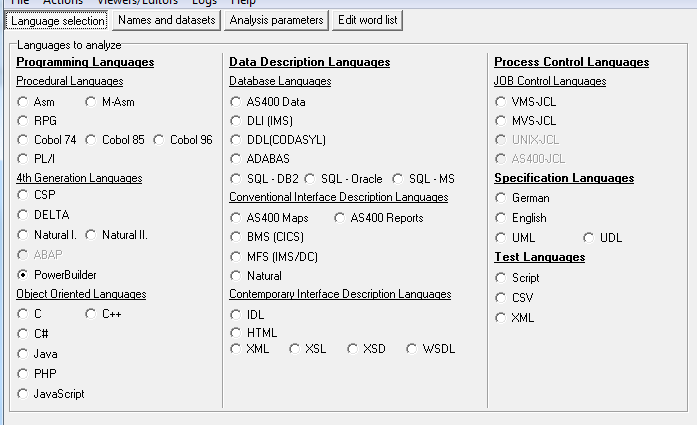
\includegraphics [width=\textwidth] {softaudit.png}
			\caption{Soft-Audit-Oberfläche zur Auswahl der Sprache die im zu vermessenden Programm verwendet wurde}
			\label{softaudit}
		\end{figure}
		Im folgenden sollen die in SoftAudit für die Vermessung von Java-Programmen verwendeten Metriken kurz beleuchtet werden. Die Formeln stammen dabei direkt von Harry Sneed, da sowohl die im Buch "`Software in Zahlen"' als auch die in der Dokumentation genannten Formeln laut seiner Aussage nicht dem aktuellen Stand des Programms entsprechen. Für einige der Metriken kann es in der Literatur abweichende Berechnungsvorschriften geben. Die hier dargestellten sind grundsätzlich die Interpretationen von Harry Sneed. Die für die Metriken verwendeten Messwerte könnten lediglich aufgezählt und mit lückenhafter Beschreibung versehen werden, da die Dokumentation und die von Herrn Sneed erhaltenen Informationen nicht für eine vollständige Aufstellung ausreichen. Aufgrund diesem Umstand und der großen Menge von durch SoftAudit ermittelten Werte wird daher darauf verzichtet und sie finden lediglich Erwähnung in den für die Metriken angegebenen Formeln. Die weiteren Funktionen von SoftAudit werden hier ebenfalls nicht erläutert, da sie im Rahmen der Aufgabenstellung keine Rolle spielen. \newline
		\subsection{Quantitätsmetriken}
			\textbf{Object Points:} Ist eine alternative zu den in der Praxis häufig verwendeten Function Points mit Fokus auf objektorientierte Sprachen und ist die gewichtete Summe der zentralen Code-Elemente.
			\begin{equation}
				\small{Object Points = (Classes * 4) + (Methods * 3) + (Interfaces * 2) + Variables}
			\end{equation}
			\textbf{Data Points:} Ebenfalls eine alternative oder Ergänzung zu Function Points deren Fokus auf den in der Software verarbeiteten Daten liegt.
			\begin{equation}
				\small{Data Points = Variables + 4 * (Views + Reports + Panels + Files + Databases)}
			\end{equation}
			\textbf{Function Points:} Gängige Methode zur Abschätzung der Größe einer Software. Kann sowohl aus Entwurfsdokumenten als auch aus dem Code ermittelt werden. Die Gewichtungs-Parameter a, b und c sind abhängig von der ermittelten durchschnittlichen Komplexität des Programms (siehe Tabelle \ref{weighting}.
			\begin{equation}
				\small{Function Points = (Databases * a) + (Files * b) + (Panels * c) + (Reports * c)}
			\end{equation}
			\begin{table} [h]
				\centering
				\tabulinesep=1mm
				\begin{tabu}{|c|c|c|c|}
					\hline
  					& $Complexity > 0.6$ & $Complexity > 0.4$ & $Complexity <= 0.4$\\
  					\hline
  					\textbf{a} & 15 & 10 & 7\\
  					\hline
  					\textbf{b} & 10 & 7 & 5\\
  					\hline
  					\textbf{c} & 7 & 5 & 4\\
  					\hline 
  				\end{tabu}
  				\caption{Wichtungsparameter für die Function-Point-Berechnung}
					\label{weighting}   
  			\end{table}
		\subsection{Komplexitätsmetriken}
			\textbf{Datenkomplexität} orientiert sich an der "`Q-Complexity"' von Chapin (1977), und stellt eine gewichtete Summe der verschiedenen Variablenreferenzen normiert durch die gesamte Zahl von Referenzen und Anweisungen dar.
			\begin{equation}
				\small{Data Complexity = \dfrac{(2 * Predicates) + (1.5 * Results) + Arguments + (0.5 * Parameter)}{Statements + References}} 
			\end{equation}
			\textbf{Datenflusskomplexität} orientiert sich an der "`Referential Complexity"' von Elshof (1976). Sie drückt das Verhältnis zwischen der Anzahl von deklarierten Daten und ihren Referenzen aus. 
			\begin{equation}
				\small{Data Flow Complexity = 1 - \dfrac{Variables * 2}{References}} 
			\end{equation}
			\textbf{Datenzugriffskomplexität} orientiert sich am "`Datenzugriffsmaß"' von Card (1991) und drückt das Verhältnis zwischen externen Datenquellen (Datenbanken und Dateien) und den Programmzugriffen auf diese aus.
			\begin{equation}
				\small{Data Access Complexity = 1 - \dfrac{Files + Databases}{Files + Databases + FileAccesses + DatabaseAccesses}} 
			\end{equation}
			\textbf{Schnittstellenkomplexität} orientiert sich am von Henry (1981) vogestellten Modell und summiert die Anzahl der Programmschnittstellen in Form von Methodenaufrufen die nicht im Programm deklariert sind gemessen an der gesamten Menge von Methodenaufrufen.
			\begin{equation}
				\small{Interface Complexity = \dfrac{ForeignMethodCalls}{MethodCalls}} 
			\end{equation}
			\textbf{Ablaufkomplexität} stellt eine normierte Variante der "`zyklomatischen Komplexität"' von McCabe (1976) dar und ist das Verhältnis von Knoten und Kanten im Kontrollflussgraphen des Programms.
			\begin{equation}
				\small{Control Flow Complexity = \dfrac{Branches - (Ifs + Switches + Loops + Returns)}{Branches}} 
			\end{equation}
			\textbf{Entscheidungskomplexität} orientiert sich an der "`Entscheidungsdichte"' von McClure (1986) und misst das Verhältnis von Kontrollflussanweisungen zu Methoden und Prozeduren.
			\begin{equation}
				\small{Conditional Complexity = \dfrac{Ifs + Switches + Cases + Loops + 1}{(4 * Methods) + (8 * Procedures)}} 
			\end{equation}
			\textbf{Beziehungskomplexität} ist ein von Harry Sneed selbst vorgeschlagenes Maß, welches verzweigende Anweisungen gemessen an der Gesamtzahl von Anweisungen darstellt.
			\begin{equation}
				\small{Branching Complexity = \dfrac{2 * (ForeignMethodCalls + Returns) + MethodCalls}{Statements}} 
			\end{equation}
			\textbf{Sprachkomplexität} ist eine modifizierte Variante des "`Volumina-Maßes"' von Halstead (1977). Sie drückt das Verhältnis von verschiedenen Sprachelementen (Anweisungs- und Daten-Typen) und der Gesamtmenge verwendeter Sprachelemente aus.
			\begin{equation}
				\small{Language Complexity = \dfrac{\dfrac{StatementTypes}{Statements} + \dfrac{DataTypes}{Variables  + Constants + Defines}}{2}} 
			\end{equation}
			\textbf{Durchschnittliche Komplexität:} Aus allen acht Komplexitätsmetriken wird abschließend der Durchschnitt errechnet. In der Dokumentation von SoftAudit ist zwar von einem gewichteten Mittelwert die Rede, tatsächlich werden in SoftAudit allerdings alle Metriken gleich gewichtet.
		\subsection{Qualitätsmetriken}
			\textbf{Sicherheit} ist im Kontext von SoftAudit als die Menge sicherer Anweisungen im Verhältnis zu allen Anweisungen definiert. Sichere Anweisungen sind dabei alle Anweisungen die keines der Folgenden Risiko-Konstrukte enthalten: 
			\begin{itemize}
				\item Duplizierte Konstruktoren
				\item ungeprüfte Rückgabewerte von Methoden
				\item Klassenvariablen die als public deklariert sind
				\item erbende Klassen die nicht als final deklariert sind
				\item ungeprüfte Parameter in Methoden die als public deklariert sind
				\item Anweisungen die SQL-Anweisungen enthalten
				\item Vergleich eines Objekts mit einem Literal
				\item serializable Klassendeklaration
				\item clonable Klassendeklaration
				\item Variablen-Casting
			\end{itemize}
			\begin{equation}
				\small{Security = \dfrac{SecureStatements * \dfrac{5}{6}}{Statements}} 
			\end{equation} 
			\textbf{Konformität} ist das Verhältnis von Regelverletzungen (gewichtet nach Schwere) zu Anweisungen. Die Auswahl der Regeln kann vom Benutzer vorgenommen werden. Wie bereits Beschrieben gibt es kein allgemeingültiges Regelwerk, sodass hier auf eine Auflistung verzichtet wird. Harry Sneed verwendet hierfür den Begriff "`Deficiencies"', in der Formel zur besseren Lesbarkeit mit "`D"' abgekürzt.
			\begin{equation}
				\small{Conformity = 1 - \dfrac{(SecurityD * 2) + (MajorD * 1,5) + MediumD + (MinorD * 0.5)}{Statements}} 
			\end{equation} 
			\textbf{Flexibilität} oder Datenunabhängigkeit bezeichnet den Grad zu dem im Code Literale und Konstanten eingebettet sind, wiederum gemessen an der Anzahl der Anweisungen.
			\begin{equation}
				\small{Flexibility = 1 - \dfrac{Literals + Constants}{Statements}} 
			\end{equation}
			\textbf{Testbarkeit} sagt aus wie viele Testfälle relativ zur Programmgröße benötigt werden. Dies wird maßgeblich durch die Anzahl der Pfade durch das Programm und die in Bedingungen verwendeten Variablen (Predikate) bestimmt. 
			\begin{equation}
				\small{Testability = \dfrac{(1 - \dfrac{Branches * 2}{Statements}) + (1-\dfrac{Predicates * 2}{References})}{2}} 
			\end{equation} 
			\textbf{Wiederverwendbarkeit} wird dadurch bestimmt in welchem Maße Methoden wiederverwendbar sind. Dies ist der Fall wenn sie keine Abhängigkeit von anderen Code-Komponenten besitzen, also keine Vererbten Komponenten der Superklasse nutzen und keine Fremdmethodenaufrufe enthalten.
			\begin{equation}
				\small{Reusability = \dfrac{ReusableMethods}{Methods + Procedures}} 
			\end{equation} 
			\textbf{Portabilität} oder Übertragbarkeit ist das Maß wie abhängig Code-Komponenten von ihrer Umgebung sind, also Datenbanken, Dateien und andere Umgebungsspezifische Elemente nutzen.
			\begin{equation}
				\small{InOutOperations = Inputs + Outputs + FileAccesses + DatabaseAccesses} 
			\end{equation} 
			\begin{equation}
				\small{InOutElements = Files + Reports + Panels + Databases} 
			\end{equation} 
			\begin{equation}
				\small{Portability = 1 - \dfrac{(FrameworkMethods * 2) + (InOutOperations * 4) + (InOutElements * 8)}{Statements}} 
			\end{equation} 
			\textbf{Modularität} sagt aus inwiefern der Code in sinnvoll zusammenhängende Bestandteile zerlegt ist (Kohäsion), in welchem Maße diese miteinander verbunden sind (Kopplung) und ob diese eine vernünftige Größe besitzen (Modulgröße).
			\begin{equation}
				\small{Cohesion = \dfrac{(Classes * 4) + (Methods * 2) + (Procedures * 2)}{(Imports * 4) + Variables}} 
			\end{equation} 
			\begin{equation}
				\small{Coupling = 1 - \dfrac{ForeignMethodCalls}{MethodCalls + Methods}} 
			\end{equation}
			\begin{equation}
				\small{ModuleSizeRating = \dfrac{Statements}{SourceFiles * OptimalModuleSize}} 
			\end{equation} 
			\begin{equation}
				\small{Modularity = \dfrac{Cohesion + Coupling + ModuleSizeRating}{3}} 
			\end{equation}  
			\textbf{Wartbarkeit} wird grundsätzlich durch die Abwesenheit von Komplexität und einer Möglichst hohen Qualität bezüglich der anderen Qualitätsmerkmale begünstigt und ergibt sich daher aus den anderen Metriken.
			\begin{equation}
				\small{Maintainability = \dfrac{(1 - AverageComplexity) + \dfrac{\sum_{}{} OtherQualityMetrics}{7}}{2}} 
			\end{equation} 
			\textbf{Durchschnittliche Qualität:} Analog zu den Komplexitätsmetriken wird abschließend auch aus allen Qualitätsmetriken ein ungewichteter Durchschnitt berechnet. 
     \section{SonarQube}
     	Die Code-Qualitäts-Plattform SonarQube bietet eine Vielzahl von Sichtweisen auf die Qualität der vermessen Software (Mit Ausnahme der Metriken die SoftAudit bietet) und deckt dabei die "`sieben Achsen"' der Softwarequalität ab \cite{SonarQubeInAction}:
     	\begin{itemize}
     		\item Fehler (Bugs)
     		\item Codierungsregeln
     		\item Testabdeckung
     		\item Codeduplikation
     		\item Schnittstellendokumentation
     		\item Komplexität (nach McCabe)
     		\item Architektur
		\end{itemize}     	
		Dabei lässt es sich in gängige Entwicklungsumgebungen und Build-Server integrieren, wodurch mit minimalem Aufwand eine kontinuierliche Vermessung der Software während der Entwicklung erfolgen kann und neben der Momentaufnahme auch Entwicklungen und Trends ersichtlich werden. \newline
		Da SonarQube ein OpenSource-Projekt ist und über den auch in dieser Arbeit verwendeten Plugin-Mechanismus fast beliebig erweiterbar ist, sei es um weitere Messwerte, andere Programmiersprachen und vieles mehr ist es ein sehr vielseitiges Werkzeug für Qualitätsmanagement. Es ist damit sowohl für kommerzielle Großprojekte als auch für studentische Arbeiten und Forschungsprojekte ein interessantes Werkzeug. \newline
		Die Web-Oberfläche von SonarQube lässt sich sehr differenziert konfigurieren und erlaubt so auch verschiedene Sichtweisen auf eine Software: für den Manager, Projektleiter, Entwickler oder Tester. Bei entsprechender Installation ist damit auch verteiltes Arbeiten über Kontinente hinweg problemlos unterstützt. Abbildung \ref{sonarqube} zeigt eine beispielhafte Projektseite mit diversen Widgets. Darüber hinaus lassen sich aber auch Übersichten über mehrere Projekte oder Detailansichten für einzelne Dateien anzeigen um beispielsweise gefundene Fehler oder Risiken genau zu lokalisieren. Auch die Regeln, die bei der Vermessung angewendet werden sollen lassen sich über die Web-Oberfläche konfigurieren. Schon mit der Standardinstallation kommen mehrere hundert Regeln die zur Verfügung stehen und entsprechend dem für das Projekt geltenden Standards ausgewählt und angepasst werden können.
		\begin{figure} [h]
				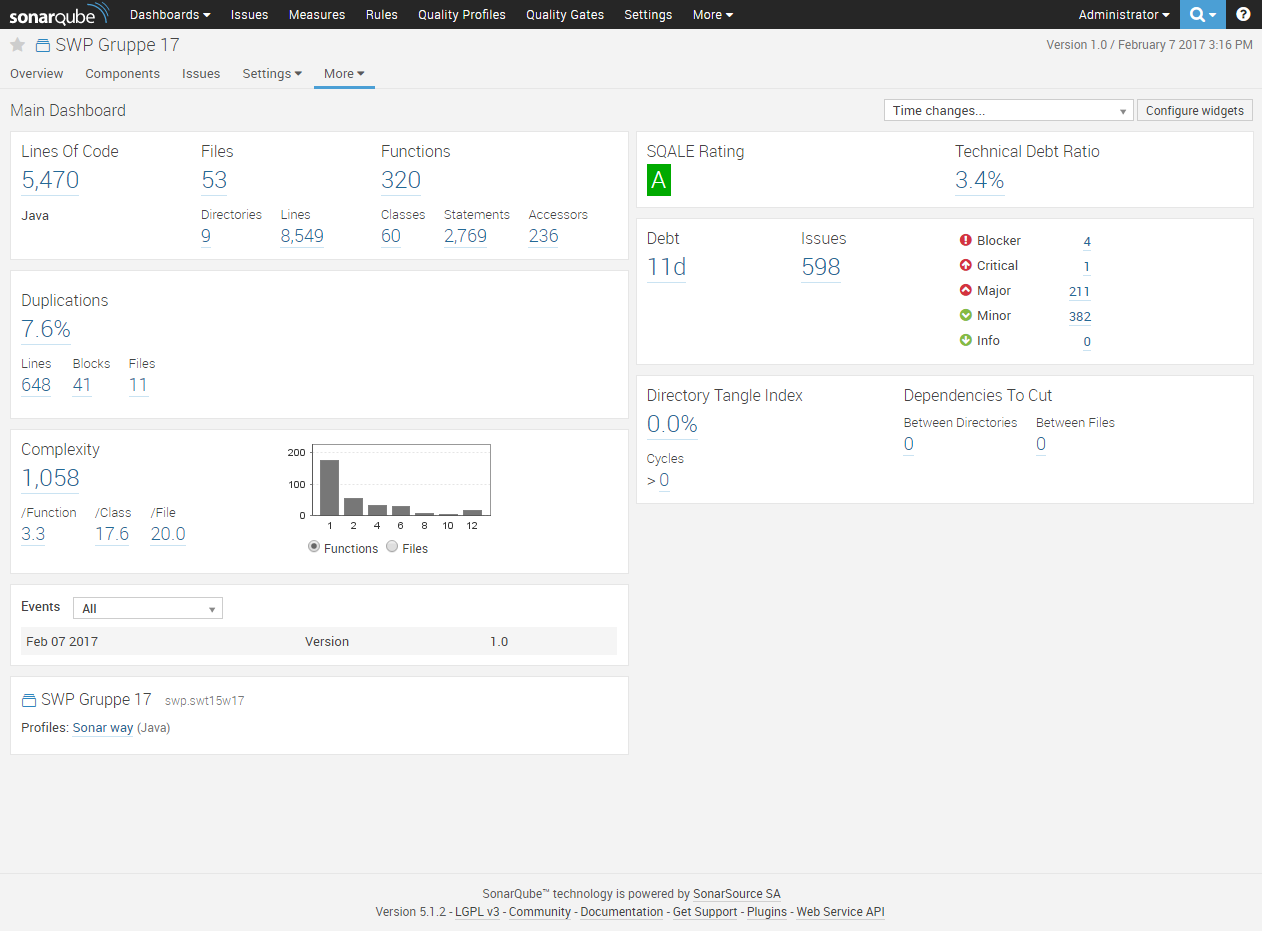
\includegraphics [width=\textwidth] {sonarqube.png}
				\caption{Web-Oberfläche von SonarQube 5.1.2 nach Vermessung eines Softwarepraktikum-Projekts}
				\label{sonarqube}
		\end{figure}
	\chapter{Plugin-Entwicklung}
		Die Implementierung des SonarQube-Plugins ist der zentrale Gegenstand der Arbeit und soll im folgenden detailliert beschrieben werden. Ausgehend von den Ansatzpunkten der von SonarQube bereit gestellten Schnittstellen zur Plugin-Entwicklung über die schrittweise Ermittlung der Metriken für die zu scannende Software bis zur Darstellung in der SonarQube-Oberfläche im Webbrowser als Widget. Als Ausgangsbasis für dieses Plugin diente ein simples Beispiel das mit Hilfe eines Tutorials den schnellen Einstieg in die Funktionsweise vom SonarQube-Plugin-Mechanismus bietet \cite{PluginTutorial}. \newline
		Dieses Kapitel bezieht sich ausschließlich auf Version 5.1.2 von SonarQube die im Juli 2015 veröffentlicht wurde. Seit dieser Version wurden diverse Änderungen an der Schnittstelle für Plugins vorgenommen \cite{APIChanges}. Besonders hervor zu heben ist dabei Version 5.2 mit der sich die Funktionsweise grundsätzlich geändert hat, sodass das entwickelte Plugin nicht aufwärts-kompatibel ist und bei Umstellung auf eine neuere SonarQube-Version das Plugin aufwendig angepasst werden müsste. Der Quellcode-parsende Teil und die Komponenten des erzeugten Code-Modells könnten zwar weitestgehend unverändert übernommen werden, die restlichen Komponenten allerdings nicht. Der Grund für die Verwendung dieser veralteten Version liegt darin, dass für das Softwarepraktikum diese Version genutzt wird und in nächster Zeit keine Umstellung geplant ist. Alle Aussagen über die SonarQube-Schnittstellen lassen sich also nicht notwendigerweise auf neuere Versionen Übertragen und müssen im Kontext von Version 5.1.2 gesehen werden. Des weiteren werden nur die in dieser Arbeit genutzten Teile der SonarQube-Schnittstellen genannt, und keine vollständige Funktionsbeschreibung vorgenommen.
		\section{Die Schnittstellen zu SonarQube}
			Um ein Plugin in SonarQube installieren zu können muss es eine Klasse geben, die von "`SonarPlugin"' erbt und deren einzige Aufgabe darin besteht alle implementierten Erweiterungen für SonarQube aufzulisten. Im Fall dieses Plugins sind dies folgende:
			\begin{itemize}
			\item Eine Implementation des Interfaces "`Metrics"', welche die Deklaration sämtlicher vom Plugin zu ermittelnder Messwerte und Metriken enthält. Diese können als Liste abgefragt werden und werden mit folgenden Eigenschaften spezifiziert:
				\begin{labeling}{Description}
					\item [Type] Integer für alle Messwerte und String für Metriken, da sonst nur eine Nachkommastelle dargestellt werden kann
					\item [Key] Für den Zugriff auf die Ergebnisse in der Datenbank im Widget
					\item [Name] Name des Wertes
					\item [Description] Beschreibung des Wertes
					\item [Direction] Gibt an ob höhere Werte (Qualität) oder niedrigere Werte (Komplexität) "`besser"' sind
					\item [Domain] Kann zur Gruppierung der Werte in der Oberfläche genutzt werden
				\end{labeling}  
			\item eine Implementation des Interfaces "`Sensor"', welche die Funktionalität des Quelldatei-Parsers kapselt und für die Ermittlung der Messwerte zuständig ist. Hier besteht Zugriff auf das Dateisystem der zu vermessenden Software. Die Hauptfunktionalität des Plugins wird von hier aus aufgerufen und gesteuert: Parsen der Quelldateien, aufbauen eines Code-Modells in dem alle relevanten Konstrukte enthalten sind, und Messwert-Ermittlung im Modell. Diese drei Schritte werden im folgenden noch detailliert beschrieben. 
			\item eine Implementation des Interfaces "`Decorator"', welche Zugriff auf die zuvor durch alle in SonarQube aktiven Sensoren ermittelten Messwerte sowie Regelverletzungen hat und daraus die Metriken, das eigentliche Ziel des Plugins errechnet.
			\item eine Implementation des Interfaces "`RubyRailsWidget"', welche den zugriff auf das Plugin-Widget kapselt.
			\end{itemize} 
		\section{Parsen von Java-Quelldateien}
			Ursprünglich war das Parsen der Java-Quelldateien für diese Arbeit gar nicht vorgesehen. Es wurde davon ausgegangen, dass SonarQube die für das Errechnen der Metriken benötigten Messwerte, oder zumindest einen Großteil davon, zur Verfügung stellt. Da SonarQube den Fokus aber wie bereits beschrieben auf das Erfassen von Regelverletzungen legt ist dies nicht der Fall. Lediglich eine Hand voll Messwerte hätten verwendet werden können. Darunter die Anzahl deklarierter Klassen und Methoden, sowie die Anzahl der Anweisungen. Außerdem sind selbst diese Messwerte nur bedingt verwendbar, da sie im Vergleich zu SoftAudit anders definiert werden. \newline
			Der zweite Ansatz war den in SoftAudit verwendeten Parser von Harry Sneed wieder zu verwenden und in das Plugin einzubinden. Dies hätte den großen Vorteil gehabt, dass kein eigenes Modell vom zu analysierenden Quellcode hätte erstellt werden müssen und die Messung zu SoftAudit identisch gewesen wäre. Es wäre also eine echte Migration und keine Neuentwicklung gewesen. Allerdings hat er dies mit der Begründung, dass die Programme nicht kompatibel sind abgelehnt. Auch eine passende Drittbibliothek lies sich nicht finden. \newline
			Um an die für die Metriken erforderlichen Messwerte zu kommen war also ein Parser für Java-Code notwendig, der diesen in ein Modell überführt aus dem sich alle relevanten Größen ableiten lassen. Direkt im Code zu zählen ist nur für einige Messwerte eine Option. Dazu zählen insbesondere alle Anweisungen die sich über Schlüsselwörter wie zum Beispiel "`for"' oder "`import"' erkennen lassen. Dabei müsste dann nur ausgeschlossen werden, dass es sich um eine Kommentarzeile oder ein String-Literal handelt. Für die meisten Messwerte ist dies aber kaum möglich, da zum Beispiel die Variablendeklarationen schwer mittels Regulärer Ausdrücke zu erkennen sind. Die Bandbreite an möglichen Varianten ist einfach zu groß. \newline
			Das Parsen der Quelldateien erfolgt Schrittweise um nach und nach für die Messung überflüssige Bestandteile zu eliminieren und die relevanten zu Erkennen und als Modellelemente abzubilden. 
			\begin{enumerate}
				\item Zunächst wird der Code von allem befreit, dass die spätere Erkennung von Code-Elementen verfälschen könnte. Dies sind Alle Kommentare und String-Literale. Erstere werden einfach entfernt, da sie für die Messung keine Rolle spielen. Die Literale werden durch Anführungszeichen als Platzhalter ersetzt da zwar der Inhalt irrelevant ist, die Anzahl aber gebraucht wird. Außerdem werden in diesem Schritt noch führende, abschließende und doppelte Leerzeichen entfernt um in den nächsten Schritten nicht immer mit beliebig vielen Leerzeichen zwischen zwei Code-Wörtern rechnen zu müssen.
				\item Der zweite Schritt dient nur zur Vereinfachung des dritten Schrittes. Hier werden alle Codezeilen in einen einzelnen langen String überführt. Außerdem werden weitere für die Modell-Erstellung irrelevante Leerzeichen entfernt. Dazu zählen alle vor und hinter Steuerzeichen wie Klammern und Operatoren.
				\item Der reduzierte Code wird nun in "`Wörter"' aufgeteilt. Dabei werden alle Steuerzeichen als eigenständige Wörter betrachtet, ebenso wie zusammenhängende Buchstaben und Zahlen. In diesem Schritt werden darüber hinaus die Wörter dahingehend geprüft ob sie einem Java-Schlüsselwort entsprechen und dementsprechend gekennzeichnet in der erstellten Wortliste abgelegt. Auch findet hier eine erneute Reduktion statt: Annotationen werden durch den Platzhalter "`@"' ersetzt. Für den umgesetzten Messalgorithmus spielen sie zwar keine Rolle, dies war zu diesem Zeitpunkt der Implementierung aber noch nicht klar. Die generierte Wortliste bietet die Basis für die eigentliche Modellerstellung.
				\item Die äußere Struktur der Java-Datei wird im vierten Schritt ermittelt. Dazu zählen die package-Anweisung, alle imports sowie die Deklaration der Hauptklasse beziehungsweise des Interfaces, der Enumeration oder der Annotationsdeklaration. Diese werden als Liste von Modellkomponenten abgelegt, wobei der Inhalt der Klasse als Wortliste beibehalten wird. 
				\item Um die Modellstruktur zu verfeinern wird der Inhalt der Hauptklasse im Anschluss rekursiv auf enthaltene Methodendeklarationen sowie Innere Klassen, Interfaces, Annotationsdeklarationen und Enumerationen durchsucht und das Modell entsprechend erweitert. Im Fall von Enumerationen wird die Werteliste bereits als eigene Modellkomponente abgelegt. Außerdem wird in diesem Schritt nach Anweisungen mit anonymen Klassen gesucht, da diese sonst die folgenden Schritte stören. Die Erkennung ist allerdings recht Einfach gehalten. Komplizierte Varianten wie die Verwendung anonymer Klassen innerhalb von Kontrollfluss-Anweisungen oder mehrere anonyme Klassen innerhalb einer Anweisung würde zu Fehlern führen, die eine Korrekte Messung unmöglich machen. Eine zuverlässigere Erkennung dieser recht seltenen Konstrukte hätte einen unverhältnismäßig hohen Aufwand bedeutet.
				\item Der Sechste Schritt ist der komplizierteste und schließt die Verschachtelung der Modellkomponenten ab. Dazu müssen alle Kontrollfluss-Anweisungen wie Schleifen und Bedingungen, sowie einige weitere Anweisungstypen erkannt werden die innere Blöcke haben, oder haben können. Außerdem werden noch einige weitere einzeilige Anweisungen in Modellkomponenten überführt die sich durch bestimmte Schlüsselwörter identifizieren lassen. Im Einzelnen sind dies alle Schleifen (For, While und Do While), If-Anweisungen inklusive Else-Zweig, Switch-Anweisungen mit deren Case-Anweisungen, Try-Anweisungen inklusive Catch-, Resource- und Finally-Blöcken, Synchronized-, Return-, Throw-, Continue-, Break- und Assert-Anweisungen sowie Anonyme Codeblöcke. Dabei wird auch hier die Suche rekursiv durchgeführt um beliebige Verschachtelungen aller Anweisungstypen zu erkennen und im Modell abzubilden. 
				\item Anschließend werden die verbliebenen Wortlisten in Anweisungen aufgeteilt, was da nun keine Sonderfälle mehr auftreten können relativ einfach über das trennen der Liste an jedem Semikolon möglich ist. Damit sind im Modell keine undefinierten Wortlisten mehr enthalten und alle folgenden Schritte reichern die erkannten Komponenten nur noch mit Details an die für das Zählen einiger Messwerte erforderlich sind.
				\item Im Achten Schritt wird in allen Anweisungen nach Variablendeklarationen und Methodenaufrufen gesucht und diese als zusätzliche Listen in den entsprechenden Modellkomponenten abgelegt.
				\item Anschließend werden alle in der Quelldatei deklarierten Variablen gesammelt und in allen Anweisungen nach Referenzen dieser Variablen gesucht und wiederum als zusätzliche Liste an der jeweiligen Komponente gespeichert. 
				\item Abschließend wird noch nach Wertzuweisungen von Variablen, Vergleichsoperatoren und Anweisungstypen wie Inkrement, Methodenaufruf und anderen gesucht. All diese Verfeinerungen spielen im implementierten Messalgorithmus aber keine Rolle, da aufgrund festgelegter Vereinfachungen oder aufgetretener Ungenauigkeiten keine sinnvolle Verwendung für diese Informationen möglich war. Da es die Messung nicht negativ beeinflusst verblieb dieser Schritt trotzdem im Parser. 
			\end{enumerate}
			Obwohl der eigene Parser für das Plugin gar nicht vorgesehen war steckt hier der Löwenanteil des Implementationsaufwandes. Java bietet eine Vielzahl von Varianten, Schreibweisen und Ausnahmen für viele Anweisungstypen an die vom Parser korrekt erkannt werden müssen um zu einem konsistenten Modell zu kommen. Dazu gehören viele Konstrukte die für die Messung gar keine Rolle spielen wie zum Beispiel Label an Schleifen oder Annotationen an Methodenparametern. Mit beinahe jeder Javadatei die zu Testzwecken geparst wurde fielen weitere gültige Möglichkeiten auf mit Java zu programmieren und der Parser musste entsprechend erweitert, beziehungsweise angepasst werden. Es ist sicher, dass nicht alles was in Java möglich ist durch das Plugin korrekt erkannt werden kann. Daher ist der Schrittweise Aufruf der Parsermethoden so gestaltet, dass bei einem Fehler das bis dahin erstellte Modell trotzdem vermessen werden kann oder bei einem sehr frühen Fehler die Datei übersprungen wird und die Ausführung von SonarQube dadurch nicht beeinträchtigt wird. In einem solchen Fall können die Ergebnisse allerdings Fehlerhaft oder verfälscht sein.
		\section{Das erstellte Code-Modell}
			Das vom Parser erzeugte Modell der Java-Datei ist grundsätzlich eine Liste von Java-Komponenten, die selbst wiederum innere Listen von Java-Komponenten besitzen können. Über dieses Konstrukt wird die Verschachtelung des Codes abgebildet. Für die Messung im aktuellen Umfang des Plugins ist dies zwar nicht zwingend notwendig, für das schrittweise Parsen ist es aber essentiell und es bietet Möglichkeiten die Messung um die Verschachtelungstiefe betreffende Werte zu erweitern. Die Java-Komponenten werden durch die abstrakte Klasse "`JavaFileContent"' (siehe Abbildung~\ref{umlmodel}) repräsentiert von der die einzelnen Komponenten-Typen, die im Modell tatsächlich enthalten sind, erben. An den konkreten Komponenten-Typen hängen weitere Informationen, die für die Messung benötigt werden sobald etwas gezählt wird, dass nicht nur das simple Erfassen eines Komponenten-Vorkommens ist. An diversen Stellen wird dazu ein Code-Schnipsel als Wortliste in der Komponente abgelegt. Dies gilt zum Beispiel auch für Rückgabewerte oder Enumerations-Werte, da diese nicht notwendiger Weise nur aus einem einzelnen Wort, im Sinne der vom Parser in Schritt drei erstellten Wortliste, bestehen müssen. Generische Datentypen sind ein solcher Fall. \newline
			Das erzeugte Modell enthält nicht alle Informationen der Quelldatei und lässt sich daher auch nicht zurück konvertieren. Um weitere Messwerte in das Plugin einzupflegen müsste das Modell gegebenenfalls um weitere Komponenten-Typen oder Attribute erweitert werden. 
			\begin{figure} [h]
				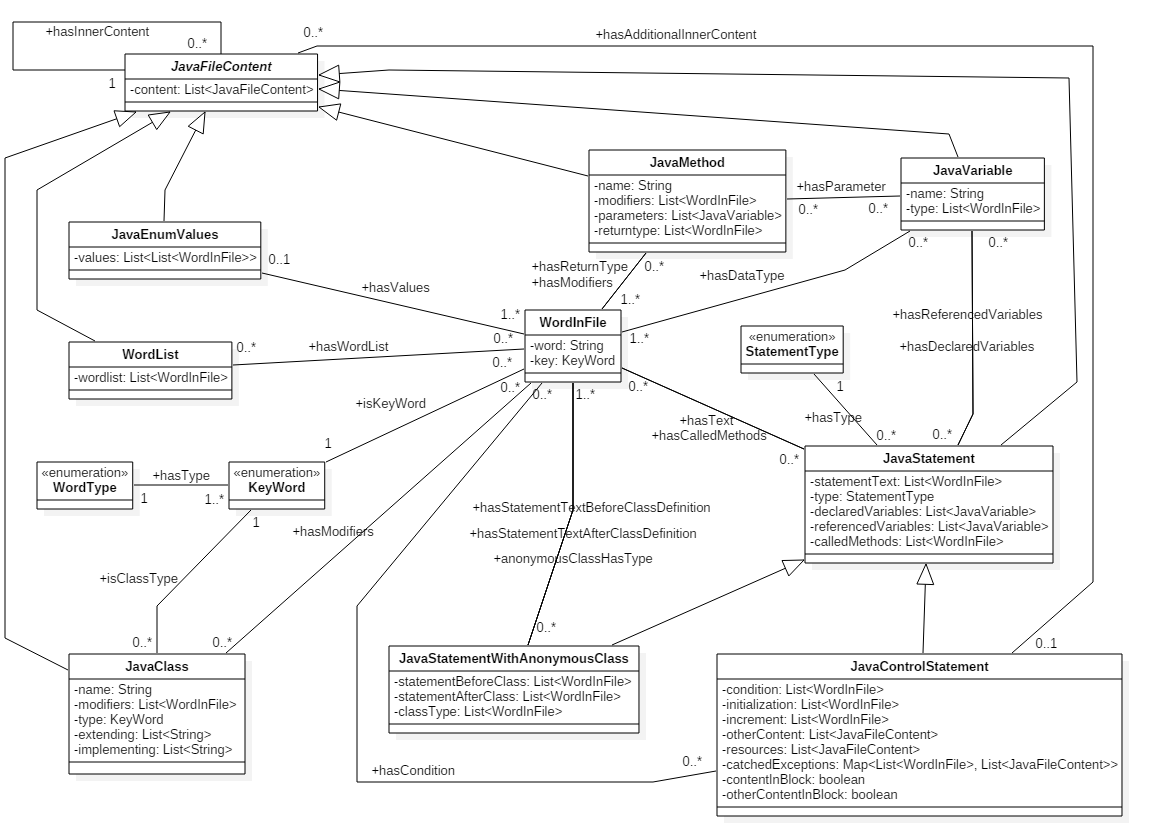
\includegraphics [width=\textwidth] {model.png}
				\caption{UML-Klassendiagramm des erzeugten Java-Code-Modells}
				\label{umlmodel}
			\end{figure}
			\subsection{Java-Datei-Komponenten}
				"`JavaFileContent"' ist die Abstrakte Oberklasse für alle Java-Datei-Komponenten. Das einzige Attribut "`content"' kapselt für Methoden, Klassen und Block-Anweisungen den inneren Code-Block. \newline \newline
				"`JavaClass"' ist die Repräsentation einer Klasse, eines Interfaces, einer Enumeration oder einer Annotations-Deklaration. Ihre Attribute ergeben sich aus der Deklarationszeile:  
				\begin{labeling} {"`otherContentInBlock"'}
					\item ["`name"'] Bezeichner der Klasse
					\item ["`modifiers"'] Liste der Modifier der Klasse
					\item ["`type"'] Klasse, Interface, Enumeration oder Annotationsdeklaration
					\item ["`extending"'] Bezeichner der Klassen von denen die Klasse erbt
					\item ["`implementing"'] Bezeichner der Interfaces die die Klasse implementiert
				\end{labeling} 
				"`JavaEnumValues"' repräsentiert eine Enumerations-Werte-Liste, deren Werte als Liste von Wortlisten im Attribut "`values"' abgelegt sind. \newline \newline
				"`JavaMethod"' kann sowohl eine Methodenimplementation als auch ein Methodeninterface sein. Im Fall eines Interfaces ist der innere Code-Block null. Die Attribute ergeben sich wiederum aus der Deklarationszeile:
				\begin{labeling} {"`otherContentInBlock"'}
					\item ["`name"'] Bezeichner der Methode
					\item ["`modifiers"'] Liste der Modifier der Methode
					\item ["`parameters"'] Liste der Methodenparameter, jeweils als JavaVariable abgelegt
					\item ["`returntype"'] Rückgabewert der Methode, als Wortliste abgelegt
				\end{labeling} 
				"`JavaStatement"' ist die allgemeine Repräsentation einer Anweisung. Im Fall von einzeiligen Anweisungen ohne inneren Code-Block ist der innere Code-Block gleich null. Die Attribute ergeben sich aus der Analyse der Anweisung. Für die Spezialfälle entfällt der Anweisungstext, da dieser in anderen Attributen aufgeschlüsselt wird. Die Listen von Variablen und aufgerufenen Methoden betreffen jeweils nicht den inneren Code-Block:
				\begin{labeling} {"`otherContentInBlock"'}
					\item ["`statementText"'] Für einzeilige Anweisungen die Anweisung als Wortliste
					\item ["`type"'] Anweisungstyp (If, While, Import, ...) 
					\item ["`declaredVariables"'] Liste der in der Anweisung deklarierten Variablen 
					\item ["`referencedVariables"'] Liste der in der Anweisung referenzierten Variablen
					\item ["`calledMethods"'] Liste der in der Anweisung aufgerufenen Methoden
				\end{labeling}
				"`JavaStatementWithAnonymousClass"' ist ein Spezialfall einer Anweisung, der sich dadurch auszeichnet, dass innerhalb der Anweisung eine anonyme Klasse verwendet wird. Der innere Code-Block ist dabei der Inhalt dieser Klasse. Die restliche Anweisung wird aufgeteilt und in den Attributen "`statementBeforeClass"', sowie "`statementAfterClass"' abgelegt. Zusätzlich wird das Interface, dass durch die anonyme Klasse implementiert wird als "`classType"' hinterlegt. \newline \newline
				"`JavaControlStatement"' ist ebenfalls ein Spezialfall der Anweisung und repräsentiert alle Anweisungen, die den Kontrollfluss des Programms steuern und / oder durch Schlüsselwörter erkennbar sind. Dies sind alle die in Schritt sechs des Parsers aufgezählt wurden. Um diese Anweisungen abzubilden sind eine ganze Reihe von zusätzlichen Attributen notwendig:
				\begin{labeling} {"`otherContentInBlock"'}
					\item ["`condition"'] Bedingung für If-Anweisungen, While- und Do-While Schleifen, Termination für For-Schleifen, Deklaration für erweiterte For-Schleifen, Operand für Switch-Anweisungen und Wert für Case-Anweisungen
					\item ["`initialization"'] Schleifenvariablen-Initialisation in For-Schleifen
					\item ["`increment"'] Inkremnt in For-Schleifen
					\item ["`otherContent"'] Inhalt des Else-Zweiges einer If-Anweisung und Inhalt des Finally-Blocks in Try-Anweisungen
					\item ["`resources"'] Resource-Block in Try-Anweisung mit Resourcen
					\item ["`catchedExceptions"'] Liste der in Try-Anweisung abgefangenen Exceptions mit dem zugehörigen Catch-Block
					\item ["`contentInBlock"'] Zeigt an ob sich der innere Block in geschweiften Klammern befindet wenn dies optional ist
					\item ["`otherContentInBlock"'] Gibt in If-Anweisungen an ob sich der Else-Zweig in geschweiften Klammern befindet
				\end{labeling}
				"`JavaVariable"' repräsentiert eine deklarierte Variable mit ihrem Bezeichner der im Attribut "`name"' und ihren Datentyp der als Wortliste im Attribut "`type"' abgelegt werden. Als einzige Java-Komponente wird diese nicht in den Komponentenlisten abgelegt sondern nur als Variablenlisten an den Anweisungsrepräsentanten. \newline \newline
				"`WordList"' ist lediglich ein Platzhalter im unfertigen Modell um zwischen und in den bereits erkannten Komponenten verbleibende Wortlisten zu kapseln die erst in den folgenden Schritten aufgeschlüsselt werden. Ist der Parser alle zehn Schritte erfolgreich durchlaufen befindet sich diese Komponente nicht mehr im Modell. Sollte in einem späten Schritt ein Fehler auftreten, werden verbleibende Wortlisten beim Messen ignoriert um zumindest eine Teilmessung möglich zu machen.
			\subsection{Weitere Modellbestandteile}
			Zur Vervollständigung des Modells sind weitere Klassen und Enumerationen notwendig. Allen voran das "`WordInFile"', welches ein Wort in der Java-Datei repräsentiert. Dabei sind wie schon beschrieben sämtliche Steuerzeichen, Operatoren und sonstige Sonderzeichen eigenständige Wörter. Jedem dieser Wörter ist das Wort selbst als String in Form des Attributs "`word"' zugeordnet und ein Wert aus der Enumeration "`KeyWord"' als Attribut "`key"'. An vielen Stellen des Parsers und des Messalgorithmus kann so nach bestimmten Schlüsselwörtern gesucht werden und erspart String-Vergleiche. Bei festen Schlüsselwörtern kann die String-Repräsentation weggelassen werden. Die Werte der Enumeration "`KeyWord"' wiederum setzen sich zusammen aus der String-Repräsentation des Schlüsselworts und dem Wort-Typ wie zum Beispiel Modifier oder Operator. Die Worttypen sind in der Enumeration "`WordType"' aufgelistet. Ebenso die Anweisungstypen in der Enumeration "`StatementType"' deren Werte in den Instanzen von "`JavaStatement"' als Typ abgelegt werden. \newpage
			\subsection{Beispiel}
				\begin{lstlisting}[frame=single]
package the.pack;
/** Some JavaDoc. */
public class SenselessClass {
   	@SuppressWarnings("unused") // a comment
   	public static void main(String[] args) {
    	int i; int j; i++; System.out.println(i);
    }
}
				\end{lstlisting}
				\begin{labeling} {\textbf{Wortliste:}}
				\item [\textbf{Wortliste:}] package, the, . pack, ;, public, class, SenselessClass, \{, @, public, static, void, main, (, String, [, ], args, ), \{, int, i, ;, int, j, ;, i, +, +, ;, System, ., out, ., println, (, i, ), ;, \}, \}
				\end{labeling}
				\begin{figure} [!h]
					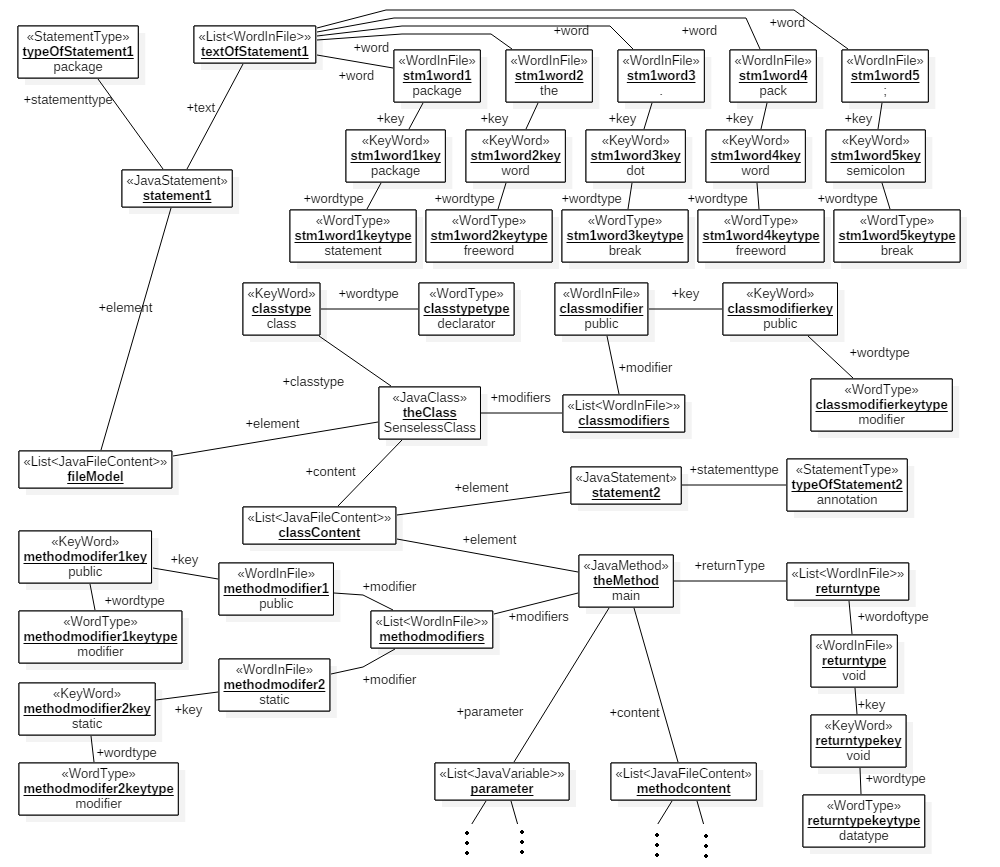
\includegraphics [width=\textwidth] {instance.png}
					\caption{Ausschnitt des für den Beispiel-Code erstellten Java-Code-Modells}
				\end{figure}
		\section{Messen der benötigten Werte}
			Nach Abschluss der zehn Parser-Schritte liegt für jede Datei eine Wortliste und ein Dateimodell vor um die Messung durchzuführen. Diese erfolgt für jede Quelldatei separat bis auf zwei Ausnahmen für Werte die nicht aufsummiert werden. Dies sind die Anzahl der Anweisungstypen und die Anzahl der Datentypen. Beide Mengen werden über den gesamten Messprozess vorgehalten um keine Typen die in mehreren Dateien verwendet werden doppelt zu zählen. Diese Werte werden der Ergebnismenge nach Abschluss aller Dateimessungen gesondert hinzugefügt. Eine weitere Ausnahme bietet der Wert für die optimale Modulgröße. Dieser ist eigentlich kein Messwert, sondern eine vom Anwender vorgegebene Größe die aus der SonarQube-Konfiguration eingelesen wird und ansonsten mit dem von Harry Sneed vorgeschlagenem Wert 200 belegt ist.\newline
			Vor der eigentlichen Messung werden alle in der zu vermessenden Software deklarierten Methoden gesammelt und als Liste ihrer Bezeichner vorgehalten. Dies ist notwendig um entscheiden zu können ob ein Methodenaufruf innerhalb der Software stattfindet, oder ob es sich um einen Fremdmethodenaufruf in ein Framework oder eine Drittbibliothek handelt. \newline
			Zwei der Messwerte werden in der Wortlisten-Repräsentation der Quelldatei vorgenommen, da im Code-Modell die Suche sehr viel aufwändiger wäre oder Daten sogar verloren gegangen sind. Dies sind die Anzahl der Literale und die Anzahl der Konstanten. Beide sind in der erzeugten Wortliste leicht anhand der Schlüsselwortzuordnung erkennbar und damit zählbar. \newline
			Alle anderen Messwerte werden durch rekursives Iterieren über das Code-Modell ermittelt indem die vorgefundenen Java-Komponenten mit ihren Attributen entsprechend der in Tabelle~\ref{messwerte} dargelegten Messwertdefinitionen ausgewertet werden. 
			\begin{center}
				\tabulinesep=1.5mm
				\begin{longtabu}{|p{0.25\textwidth}|c|p{0.6\textwidth}|}
					\hline
  					\textbf{Messwert} & \textbf{ID} & \textbf{Definition} \\
  					\hline
    				Quelldateien & SRC & Anzahl vermessener Dateien (Parsen bis mindestens Schritt fünf erfolgreich)\\
    				\hline
    				Deklarierte Klassen & CLA & Alle deklarierten Klassen, auch innere und anonyme Klassen unabhängig von der Sichtbarkeit \\
    				\hline
    				Deklarierte Interfaces & INT & Alle deklarierten Interfaces, Enumerationen und Annotationen \\
    				\hline
    				Deklarierte nicht private Methoden & MET & Alle deklarierten Methoden und Methodeninterfaces ohne den Modifier "`private"' ohne Getter und Setter \\
    				\hline
    				Deklarierte private Methoden & PME & Alle deklarierten Methoden und Methodeninterfaces mit dem Modifier "`private"' ohne Getter und Setter \\ 
    				\hline
    				Wiederverwendbare Methoden & RUM & Alle deklarierten Methoden, die keine Fremdmethodenaufrufe enthalten \\
    				\hline
    				Methodenaufrufe & FUC & Alle Methodenaufrufe außer Aufrufe von als Getter oder Setter erkannten Methoden im Projekt \\
    				\hline
    				Fremdmethodenaufrufe & FFC & Alle Aufrufe von Methoden die nicht im Projekt deklariert sind \\
    				\hline
    				Imports & IMP & Alle Import- und Package-Anweisungen \\
    				\hline
    				Anweisungen & STM & Alle Anweisungen: Methoden-, Interface- und Enumerations-Deklarationen, Enumerations-Wertelisten, Kontrollflussanweisungen (If, Schleifen, ...), und alle anderen Anweisungen die durch ein Semikolon abgeschlossen werden \\
    				\hline
    				Anweisungstypen & STY & Alle Kontrollflussanweisungstypen und Schlüsselwort bedingte Anweisungstypen zählen nur einmal, alle anderen Anweisungen zählen als eigener Typ \\
    				\hline
    				If-Anweisungen & IFS & Alle If- und Try-Anweisungen, Else-Zweige sowie Finally- und Catch-Blöcke zählen nicht mit \\
    				\hline
    				Schleifen & LOP & Alle For-, While- und Do-While-Anweisungen \\
    				\hline
    				Switch-Anweisungen & SWI & Alle Switch-Anweisungen \\
    				\hline
    				Case-Anweisungen & CAS & Alle Case-Anweisungen, inklusive dem Default-Case. \\
    				\hline
    				Return-Anweisungen & RET & Alle Return-Anweisungen \\
    				\hline
    				Kontrollfluss-Zweige & BRA & Ein Zweig je Return- und Case-Anweisung sowie Catch-Block, Zwei Zweige je If-, For-, While-, Do-While- und Try-Anweisung \\
    				\hline
    				Deklarierte Variablen & VAR & Alle deklarierten Variablen, unabhängig vom Ort der Deklaration und der Sichtbarkeit \\
    				\hline
    				Globale Variablen & GVA & Alle deklarierten Klassen-Variablen \\
    				\hline
    				Datentypen & DTY & Alle für Variablen, Parameter und Rückgabewerte verwendeten Datentypen \\
    				\hline
    				Variablenreferenzen & REF & Alle Vorkommen von Variablen-Bezeichnern inklusive Methodenparameter \\
    				\hline
    				Parameter & PAR & Alle Methodenparameter \\
    				\hline
    				Predikate & PRE & Variablenreferenzen in Bedingungen von Kontrollflussstatements (If, Schleifen, Switch, ...) \\
    				\hline
    				Argumente und Ergebnisse & ARG & Alle Variablenreferenzen die nicht Parameter oder Predikat sind \\
    				\hline
    				Konstanten & CON & Werte von Enumerationen und Zahlen im Code \\
    				\hline
    				Literale & LIT & Alle String-Literale im Code \\
    				\hline
    				Optimale Modulgröße & OMS & Ideale Größe einer Quelldatei in Anweisungen \newline(Standard = 200) \\
    				\hline
    				\caption{Übersicht der vom Plugin ermittelten Messwerte, der intern verwendeten ID und ihrer Definition für das SonarQube-Plugin}
					\label{messwerte} \\
  				\end{longtabu}  
  			\end{center}
  			\subsection{Das Problem der Messwertdefinition}
  				Neben dem Problem, dass Java eine Vielzahl von Sprachkonstrukten mit diversen Ausnahmen und Sonderregeln bietet, die den Parser sehr komplex machen war die Frage nach der Definition der Messwerte die größte Schwierigkeit während der Implementierung des Plugins. Da wie bereits beschrieben die Dokumentation von SoftAudit dies nicht ausführlich beleuchtet und schon bei sehr groben Sprachkonstrukten wie der Anzahl der deklarierten Klassen eine erstaunliche Bandbreite an Interpretationsvarianten existiert musste hier eine eigene Definition gefunden werden. \newline
  				Harry Sneed stand freundlicherweise über die gesamte Bearbeitungszeit für Fragen bezüglich der SoftAudit-Messung zur Verfügung sodass ein tieferer Einblick in SoftAudit möglich war, als es nur auf Basis der Dokumente realisierbar gewesen wäre. Trotzdem war es nicht möglich eine detaillierte und vollständige Definition der Messwerte von SoftAudit aufzustellen, oder gar konkrete Algorithmen für die Messung wieder zu verwenden. Dies liegt zum einen daran, dass für die Arbeit kein Einblick in den Quellcode von SoftAudit bestand und zum anderen, dass Harry Sneed selbst die Funktionsweise des SoftAudit-Parsers nicht mehr in Gänze nachvollziehen konnte. Zum Teil sind durch Rückfragen auch Fehler oder fragwürdige Messwertdefinitionen gefunden worden, deren Übernahme in das SonarQube-Plugin nicht sinnvoll gewesen wäre. \newline 
  				Als Beispiel sei hier die Anzahl der deklarierten Methoden genannt. Es sind während der Implementierung eine ganze Reihe von Fragen aufgetreten die für die genaue Definition beantwortet werden mussten:
  				\begin{itemize}
  					\item Welche Rolle spielt die Sichtbarkeit, sind private Helfer-Methoden relevant für die Metriken?
  					\item Ist ein Konstruktor eine Methode?
  					\item Zählen auch die trivialen Methoden, also Getter und Setter als Methode im Sinne der Metriken?
  					\item Wenn triviale Methoden gesondert behandelt werden, wie definieren sich diese dann, über ein Namensschema und / oder die Art des Inhalts? 
  					\item Sollten Methodeninterfaces in abstrakten Klassen oder Interfaces ebenfalls mitgezählt werden?
  				\end{itemize}
  				Dabei ist diese Aufstellung noch nicht einmal vollständig. Bei noch genauerer Betrachtung der Thematik lassen sich leicht weitere Varianten finden die man gesondert behandeln könnte oder sollte. Dazu kommt das diese Fragen von verschiedenen Autoren und Messprogrammen zum Teil sehr verschieden Beantwortet werden. Jedes Software-Vermessungsprogramm hat also seine eigene Definition der Messwerte, wodurch die Ergebnisse kaum Vergleichbar sind, selbst wenn sie vom Namen her die gleichen Messwerte betrachten. Dies trifft selbstverständlich auch auf das im Rahmen dieser Arbeit entstandene SonarQube-Plugin zu. Die letztendlich gewählten Definitionen sind neben der Orientierung an SoftAudit, der Meinung des Lehrstuhls und der persönlichen Einstellung auch noch der Überlegung geschuldet welche Definition sich leichter messen lässt und keinen unverhältnismäßig hohen Aufwand für den Parser bedeutet um den Rahmen der Belegarbeit nicht zu sprengen. Daher sind alle Definitionen kritisch zu betrachten und für zukünftige Arbeiten gegebenenfalls anzupassen.   
		\section{Metriken berechnen} \label{metriccompute}
			Bevor die eigentlichen Metriken berechnet werden bezieht der SonarQube-Decorator des Plugins zusätzlich zu den vom Sensor gemessenen Werten einige von SonarQube bereits ermittelte Werte und berechnet damit auch noch ein Zwischenergebnis, das für eine Metrik benötigt wird. Diese sind in Tabelle \ref{soqumesswerte} aufgelistet. 
			\begin{table} [h]
				\centering
				\tabulinesep=1.5mm
				\begin{tabu}{|p{0.25\textwidth}|c|p{0.6\textwidth}|}
					\hline
  					\textbf{Messwert} & \textbf{ID} & \textbf{Definition} \\
  					\hline
  					Sicherheitskritische Verstöße & SED & Entspricht "`Blocker"'\\
  					\hline
  					Schwere Verstöße & MAD & Entspricht "`Critical"'\\
  					\hline
  					Mittlere Verstöße & MED & Entspricht "`Major"'\\
  					\hline 
  					Leichte Verstöße & MID & Entspricht "`Minor"'\\
					\hline  				
					Sichere Anweisungen & SST & Anzahl Anweisungen - Sicherheitskritische Verstöße \\
					\hline 
  				\end{tabu}
  				\caption{Von SonarQube bereitgestellte Messwerte bezüglich Regelverletzungen}
					\label{soqumesswerte}   
  			\end{table}
  			\newline
			Da auf die in SoftAudit verwendeten Metriken bereits in Kapitel \ref{Kapitel2} eingegangen wurde, werden hier nur die Abweichungen davon erwähnt. Ansonsten folgt die Berechnung den dort genannten Formeln und die Abweichungen der Messergebnisse resultieren ausschließlich aus den abweichenden Messwertdefinitionen oder abweichenden Messalgorithmen. Zur besseren Lesbarkeit der Formeln werden anstatt der Metrikbezeichnungen, die im Programm als ID verwendeten Abkürzungen verwendet. Die Zuordnung ist der Tabelle \ref{metriken} zu entnehmen.
			\begin{table} [h]
				\centering
				\tabulinesep=1.5mm
				\begin{tabu}{|l|c||l|c|}
					\hline
  					\textbf{Metrik} & \textbf{ID} & \textbf{Metrik} & \textbf{ID} \\
  					\hline
    				Object Points & OBP & & \\
    				\hline
    				\textbf{Komplexitätsmetriken} & & \textbf{Qualitätsmetriken} & \\
    				\hline
    				Datenkomplexität nach Chapin & DCO & Modularität & MOD \\
    				\hline
    				Datenflusskomplexität nach Elshof & DFC & Testbarkeit & TST \\
    				\hline
    				Schnittstellenkomplexität nach Henry & ICO & Wiederverwendbarkeit & REU \\
    				\hline
    				Ablaufkomplexität nach McCabe & CFC & Sicherheit & SEC \\
    				\hline
    				Entscheidungskomplexität nach McClure & COC & Flexibilität & FLE \\
    				\hline
    				Beziehungskomplexität nach Sneed & BRC & Konformität & COF \\
    				\hline
    				Sprachkomplexität nach Halstead & LCM & Wartbarkeit & MAI \\
    				\hline
    				Durchschnittliche Komplexität & ACM & Durchschnittliche Qualität & AQM \\
    				\hline
  				\end{tabu}
  				\caption{Übersicht der vom Plugin errechneten Metriken und Zuordnung zur  ID}
					\label{metriken}   
  			\end{table}
  			\newline
  			Auf Basis der Aussage, dass im Java-Kontext Prozeduren nicht existieren sondern alles Methoden sind wurden diese Metrikbestandteile entfernt. Auf vier Metriken die in SoftAudit berechnet werden wird vollständig verzichtet. Dies ergibt sich daraus, dass für diese Metriken eine verhältnismäßig große Zahl an zusätzlichen Messwerten notwendig wären (zehn) die zum Teil eine erhebliche Erweiterung des Parsers notwendig gemacht hätten und damit im Rahmen dieser Arbeit zu aufwendig gewesen wären. Dies sind in erster Linie alle Messwerte die sich auf Ein- und Ausgaben beziehungsweise Datei- und Datenbank-Zugriffe beziehen. Dies betrifft die Datenzugriffskomplexität nach Card, die Portabilität, die Data Points und die Function Points. Dadurch ergeben sich für die drei folgenden Metriken abweichende Berechnungsformeln, wobei die einzige Änderung darin besteht, dass für Durchschnittsermittlungen die fehlende Metrik weggelassen, und der Dividend entsprechend angepasst wird: 
			\begin{itemize}
				\item Durchschnittliche Komplexität:
				\begin{equation}
					\small{ACM = \dfrac{DCO + DFC + ICO + CFC + COC + BRC + LCM}{7}}
				\end{equation}
				\item Wartbarkeit:
				\begin{equation}
					\small{MAM = \dfrac{(1 - ACM) + \dfrac{MOD + TST + REU + SEC + FLE + \dfrac{COF} {2}}{6}}{2}}
				\end{equation}
				\item Durchschnittliche Qualität:
				\begin{equation}
					\small{AQM = \dfrac{MOD + TST + REU + SEC + FLE + COF + MAM}{7}}
				\end{equation}
			\end{itemize}
			Darüber hinaus wurden einige Metriken angepasst um auf deutlich abweichende Messwerte oder fehlende Messwerte zu reagieren. Dies ist insofern als zulässig zu betrachten, da eine veränderte Messwertdefinition auch Veränderungen in den Metriken hervorrufen kann, in denen dieser Messwert verwendet wird. 
			\begin{itemize}
				\item Object Points: Es werden nur Globale Variablendeklarationen berücksichtigt
				\begin{equation}
					\small{OBP = (CLA * 4) + (MET * 3) + (INT * 2) + GVA}
				\end{equation}
				\item Datenkomplexität: Notwendige Anpassung durch Zusammenfassung der Messwerte Argumente und Ergebnisse:
				\begin{equation}
					\small{DCO = \dfrac{(PRE * 2) + (ARG * 1,25) + (PAR * 0,5)}{STM + REF}}
				\end{equation} 
				\item Beziehungskomplexität: Notwendige Anpassung durch deutlich abweichende Ergebnisse bei der Messung der Fremdmethodenaufrufe 
				\begin{equation}
					\small{BRC = \dfrac{(FFC * 2) + (RET * 2) + (FUC - FFC)}{STM * 2}}
				\end{equation}
				\item Sprachkomplexität: Zur Vereinfachung wurde die Anzahl der definierten Makros im Code weggelassen
				\begin{equation}
					\small{ACM = \dfrac{\dfrac{STY}{STM} + \dfrac{DTY}{VAR + CON}}{2}}
				\end{equation}
			\end{itemize}
			Abschließend wird für alle Metriken, mit Ausnahme der Object Points vor der Durchschnittsberechnung eine Normalisierung vorgenommen, da Aufgrund der Abweichenden Messwertermittlung zum Teil Werte größer als eins errechnet werden, was die Durchschnittswerte verfälscht. Daher werden alle Werte größer eins oder kleiner null auf eins, beziehungsweise null gesetzt. Diese Werte sind als Grenzwerte zu betrachten.
		\section{Darstellung im SonarQube-Widget}
			Die Darstellung in der Web-Oberfläche von SonarQube erfolgt über ein RubyRailsWidget das über die SonarQube-Administration einem Dashboard hinzugefügt werden kann und eine Auswahl der ermittelten Messwerte und sämtliche Metriken in Form einfacher Tabellen darstellt. Die Formatierung der Messwerte und Metrik-Ergebnisse wird dem SonarQube-Standard-Formatierer überlassen was leider zur Folge hat, dass für Metriken die ermittelten Werte als formatierte Strings abgelegt werden müssen, da sonst nur eine Nachkommastelle dargestellt werden kann. Dies würde die Aussagekraft der Metriken massiv einschränken da die meisten Veränderungen während der Projektlaufzeit und auch viele Unterschiede zwischen zwei Programmen erst mit der zweiten und dritten Nachkommastelle sichtbar werden. Dies blockiert allerdings eine Trend-Anzeige im Vergleich mit vorherigen Messungen. In einer späteren Version von SonarQube wurde das Problem behoben. In Abbildung \ref{widget} ist die Widget-Darstellung in einer lokalen SonarQube-Installation zu sehen mit der ein Softwarepraktikumsprojekt aus dem Jahr 2015 beispielhaft vermessen wurde.\newline
			\begin{figure} [h]
				\centering
				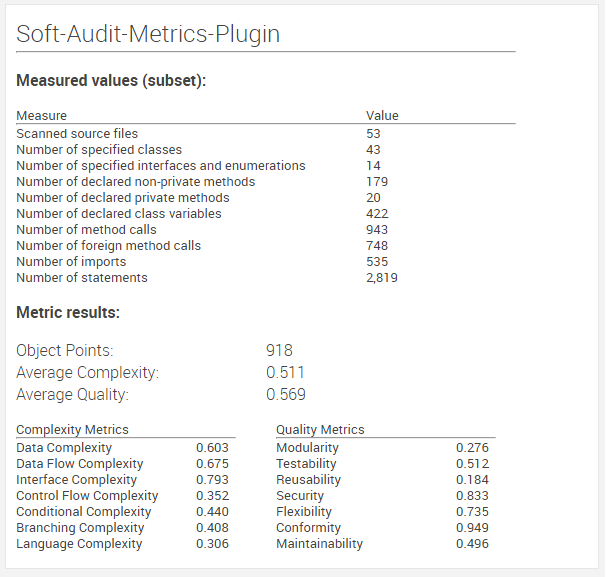
\includegraphics [width=0.6\textwidth] {widget.png}
				\caption{Plugin-Widget in SonarQube-Oberfläche}
				\label{widget}
			\end{figure}
			Des weiteren wird eine Log-Datei erzeugt die abhängig von der Plugin-Konfiguration die Zwischenschritte oder nur die Ergebnisse der Vermessung enthält. Diese Ausgabe wurde hauptsächlich zu Testzwecken benötigt, kann aber auch im produktivem Einsatz genutzt werden um Ergebnisse nachzuvollziehen. Abbildung \ref{logfile} zeigt die Ergebnisausgabe zur Messung die auch im Widget zu sehen ist.
			\begin{figure} [h]
				\centering
				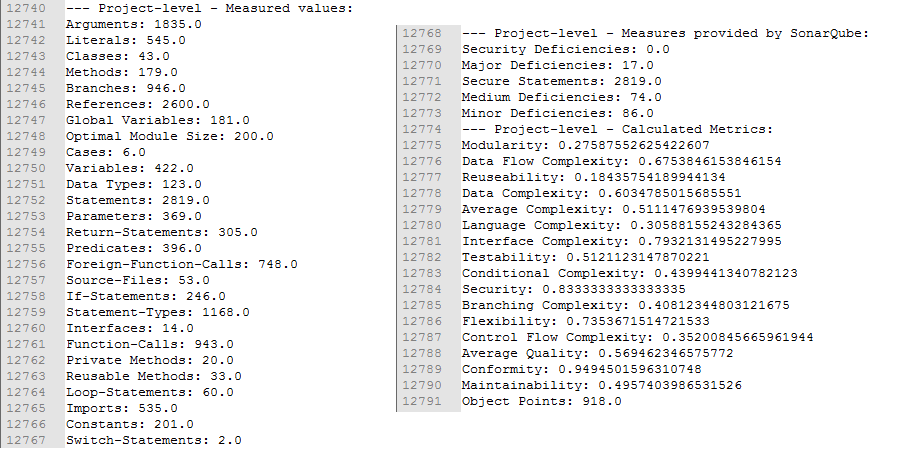
\includegraphics [width=\textwidth] {logfile.png}
				\caption{Plugin-Log-Datei für Beispielmessung}
				\label{logfile}
			\end{figure}
	\chapter{Plugin-Einsatz}
		Aus Zeitmangel war ein Test unter realen Bedingungen mit der am Lehrstuhl betriebenen Installation von SonarQube leider nicht mehr möglich. Die folgenden Ausführungen wurden daher mit einer lokalen Installation von SonarQube 5.1.2 unter Windows 7 und dem SonarScanner in Version 2.6.1, sowie der dieser Arbeit beigefügten Version 1.0 des entwickelten Plugins durchgeführt. Für die Regelverletzungen wurde das in SonarQube initial enthaltene Standard-Set verwendet, da eine vollständige Abbildung auf die von SoftAudit verwendeten Regeln nicht möglich war und das Regelwerk ohnehin von den Lehrstuhlmitarbeitern zusammengestellt werden sollte, um sicher zu stellen dass die gemessene Konformität auch auf den gewollten Standard zielt. Die Einbindung in die Lehrstuhlinstallation sollte aber aufgrund der Versionsgleichheit unproblematisch sein und die gleichen Ergebnisse liefern. Die Vergleichsmessung erfolgte mit SoftAudit in der Version 7, Release 1216, das von Harry Sneed zur Verfügung gestellt wurde.\newline
		Für die Testmessung wurden drei abgeschlossene Softwarepraktikums-Projekte aus dem Wintersemester 2015/2016 verwendet. Vermessen wurde dabei nur der Programmcode, nicht die Tests und ebenfalls nicht eventuell eingebundene Drittbibliotheken. Darüber hinaus wurden noch Testmessungen an kleineren studentischen Programmen aus dem Grundstudium, dem Quellcode des Plugins selbst und einer Auswahl von Quelldateien aus Open-Source und auch kommerziellen Projekten durchgeführt, deren Ergebnisse hier aber nicht weiter aufgeführt werden. Das Ziel dieser Messungen war in erster Linie eine möglichst große Bandbreite von Java-Code zu vermessen um eventuelle Lücken im Parser-Algorithmus und andere Fehlerquellen aufzudecken. 
		\section{Messergebnisse im Vergleich zu SoftAudit}
			Die Messergebnisse für alle drei vermessenen Projekte von SoftAudit und denen des Plugins sind in Tabelle \ref{measuretable} dargestellt. Für einige wenige Messwerte fehlt das Ergebnis von SoftAudit, da dieser Messwert nicht ermittelt wird oder nicht in der Ausgabe enthalten ist. \newline
			Es fällt auf, dass es nur bei sehr wenigen Messwerten gelungen ist zum selben Ergebnis zu kommen. In den meisten Fällen liegt dies wie schon beschrieben an den unklaren Messwertdefinitionen und Messalgorithmen die in SoftAudit verwendet werden. Recht gut funktioniert die Nachbildung der SoftAudit-Messung bei allen Kontrollfluss-Anweisungen (also Schleifen, If-Anweisungen, ...). Bei allem was Variablen und deren Nutzung betrifft ist die Annäherung dagegen besonders schlecht. Der zweite Bereich in dem die Abweichung massiv ist, sind die Regelverstöße, was wiederum auf das völlig andere Regelwerk zurückzuführen ist. Hier ließe sich mit entsprechender Regelauswahl entweder eine bessere Annäherung an SoftAudit erreichen oder aber eine der Lehrstuhlmeinung entsprechende Einschätzung der Regeln, die nicht notwendiger Weise dem Regelwerk von Harry Sneed entsprechen muss. Hierfür ist keine Anpassung des Plugins notwendig. Die Konfiguration von SonarQube über die Administrator-Oberfläche während der Laufzeit reicht aus. \newline
			\begin{table} [!p]
				\centering
				\tabulinesep=1.5mm
				\begin{tabu}{|p{0.27\textwidth}||r|r||r|r||r|r|}
					\hline
  					\multirow{2}{*}{\textbf{Messwert}} & \multicolumn{2}{c||}{\textbf{Gruppe 13}} & \multicolumn{2}{c||}{\textbf{Gruppe 17}} & \multicolumn{2}{c|}{\textbf{Gruppe 29}} \\ \cline{2-7} & SoftAudit & Plugin & SoftAudit & Plugin & SoftAudit & Plugin \\
  					\hline
  					Quelldateien & 53 & 53 & 53 & 53 & 26 & 26\\
    				\hline
    				Deklarierte Klassen & 31 & 43 & 39 & 46 & 12 & 16\\
    				\hline
    				Deklarierte Interfaces & 23 & 14 & 11 & 14 & 8 & 14\\
    				\hline
    				Nicht private Methoden & 152 & 179 & 239 & 254 & 62 & 68\\
    				\hline
    				Private Methoden & - & 20 & - & 15 & - & 5\\ 
    				\hline
    				Wiederverwendbare Met. & 93 & 33 & 197 & 61 & 55 & 9\\
    				\hline
    				Methodenaufrufe & 1046 & 943 & 2133 & 1980 & 729 & 784\\
    				\hline
    				Fremdmethodenaufrufe & 553 & 748 & 620 & 1464 & 235 & 683\\
    				\hline
    				Imports & 535 & 535 & 598 & 598 & 322 & 322\\
    				\hline
    				Anweisungen & 2926 & 2819 & 4311 & 4247 & 1393 & 1497\\
    				\hline
    				Sichere Anweisungen & - & 2819 & - & 4243 & - & 1497\\
    				\hline
    				Anweisungstypen & 1505 & 1168 & 2196 & 1964 & 715 & 762\\
    				\hline
    				If-Anweisungen & 250 & 246 & 379 & 356 & 28 & 30\\
    				\hline
    				Schleifen & 61 & 60 & 77 & 73 & 33 & 34\\
    				\hline
    				Switch-Anweisungen & 2 & 2 & 4 & 4 & 4 & 4\\
    				\hline
    				Case-Anweisungen & 6 & 6 & 23 & 23 & 19 & 19\\
    				\hline
    				Return-Anweisungen & 298 & 305 & 523 & 521 & 104 & 104\\
    				\hline
    				Kontrollfluss-Zweige & 1007 & 946 & 1468 & 1402 & 246 & 252\\
    				\hline
    				Deklarierte Variablen & 257* & 422 & 502* & 555 & 158* & 237\\
    				\hline
    				Globale Variablen & 257* & 181 & 502* & 211 & 158* & 87\\
    				\hline
    				Datentypen & 188 & 123 & 202 & 147 & 162 & 83\\
    				\hline
    				Variablenreferenzen & 2443 & 2600 & 3488 & 5158 & 1067 & 1543\\
    				\hline
    				Parameter & 267 & 369 & 614 & 668 & 245 & 228\\
    				\hline
    				Prädikate & 616 & 396 & 760 & 686 & 137 & 78\\
    				\hline
    				Argumente / Ergebnisse & 1560 & 1835 & 2114 & 3804 & 685 & 1237\\
    				\hline
    				Konstanten & 279 & 201 & 524 & 360 & 291 & 151\\
    				\hline
    				Literale & 638 & 545 & 1327 & 1139 & 405 & 346\\
    				\hline
    				Optimale Modulgröße  & 200** & 200 & 200** & 200 & 200** & 200\\
    				\hline
    				Sicherheitskr. Verstöße & 107 & 0 & 170 & 4 & 46 & 0\\
    				\hline
    				Schwere Verstöße & 114 & 17 & 270 & 1 & 51 & 1\\
    				\hline
    				Mittlere Verstöße & 636 & 74 & 1813 & 211 & 491 & 107\\
    				\hline
    				Leichte Verstöße & 1014 & 86 & 1587 & 382 & 465 & 102\\
    				\hline
  				\end{tabu}  
  				\caption{Vergleich der Messergebnisse des Plugins mit der SoftAudit-Messung \newline
  				 *: Es ist nicht ganz klar welche Variablen von SoftAudit gezählt werden. Die Zahlen entsprechen eher der Gesamtmenge. \newline
  				**: Laut Aussage von Harry Sneed. Nicht in Ausgabe enthalten.}
				\label{measuretable}
  			\end{table}
  		\section{Metrik-Resultate im Vergleich zu SoftAudit}
  			Einige Messwerte verursachten durch massive Abweichungen Probleme mit den Metriken in denen sie verwendet werden. Aus diesem Grund wurden die in Kapitel \ref{metriccompute} beschriebenen Anpassungen vorgenommen. Im einzelnen sind dies die Anzahl der deklarierten Variablen, die Fremdmethodenaufrufe, und daraus resultierend die Anzahl der Wiederverwendbaren Methoden. \newline
  			Mit den vorgenommenen Anpassungen ergeben sich aus den Messwerten die in Tabelle \ref{metricstable} dargestellten Metrik-Resultate. Die Metriken Konformität und Sicherheit sind direkt vom verwendeten Regelwerk abhängig und daher eigentlich nicht vergleichbar. Außerdem verbleiben trotz der Formel-Anpassungen in den Metriken Interface-Komplexität, Verzweigungskomplexität, Modularität  und Wiederverwendbarkeit starke Abweichungen, wodurch die Aussage der Messergebnisse eine völlig andere ist. \newline
  			\begin{table} [!h]
				\centering
				\tabulinesep=1.5mm
				\begin{tabu}{|p{0.27\textwidth}||r|r||r|r||r|r|}
					\hline
  					\multirow{2}{*}{\textbf{Metrik}} & \multicolumn{2}{c||}{\textbf{Gruppe 13}} & \multicolumn{2}{c||}{\textbf{Gruppe 17}} & \multicolumn{2}{c|}{\textbf{Gruppe 29}} \\ \cline{2-7} & SoftAudit & Plugin & SoftAudit & Plugin & SoftAudit & Plugin \\
  					\hline
  					Object Points & 883 & 918 & 1397 & 1185 & 408 & 383\\
    				\hline
    				\textbf{Komplexitätsmetriken} & \multicolumn{6}{c|}{} \\ 
    				\hline
    				Datenkomplexität & 0,617 & 0,603 & 0,571 & 0,686 & 0,509 & 0,597\\
    				\hline
    				Datenflusskomplexität & 0,789 & 0,675 & 0,712 & 0,784 & 0,703 & 0,692 \\
    				\hline
    				Schnittstellenkomplexität & 0,528 & 0,793 & 0,291 & 0,739 & 0,322 & 0,871\\
    				\hline
    				Ablaufkomplexität & 0,393 & 0,352 & 0,331 & 0,319 & 0,313 & 0,317\\
    				\hline
    				Entscheidungskomplexität & 0,404 & 0,439 & 0,463 & 0,449 & 0,272 & 0,323\\
    				\hline
    				Beziehungskomplexität & 0,791 & 0,408 & 0,787 & 0,528 & 0,862 & 0,559\\
    				\hline
    				Sprachkomplexität & 0,432 & 0,305 & 0,353 & 0,311 & 0,437 & 0,361\\
    				\hline
    				\diameter -Komplexität & 0,549 & 0,511 & 0,448 & 0,545 & 0,489 & 0,531\\
    				\hline
    				\textbf{Qualitätsmetriken} & \multicolumn{6}{c|}{} \\
    				\hline
    				Modularität & 0,486 & 0,275 & 0,519 & 0,337 & 0,522 & 0,210\\
    				\hline
    				Testbarkeit & 0,403 & 0,512 & 0,441 & 0,536 & 0,695 & 0,781\\
    				\hline
    				Wiederverwendbarkeit & 0,531 & 0,184 & 0,788 & 0,240 & 0,785 & 0,132\\
    				\hline
    				Sicherheit & 0,802 & 0,833 & 0,801 & 0,832 & 0,805 & 0,833\\
    				\hline
    				Flexibilität & 0,687 & 0,735 & 0,571 & 0,647 & 0,501 & 0,668\\
    				\hline
    				Konformität & 0,478 & 0,949 & 0,223 & 0,903 & 0,361 & 0,893\\
    				\hline
    				Wartbarkeit & 0,514 & 0,495 & 0,573 & 0,480 & 0,642 & 0,490\\
    				\hline
    				\diameter -Qualität & 0,601 & 0,569 & 0,573 & 0,568 & 0,642 & 0,572\\
    				\hline
  				\end{tabu}  
  				\caption{Vergleich der Metrik-Resultate des Plugins mit der SoftAudit-Messung}
				\label{metricstable}
  			\end{table}
			\newline Wenn man als Endergebnis nur die Durchschnittswerte für Komplexität und Qualität sowie die Object Points betrachtet lassen sich folgende Aussagen aus dem Vergleich ableiten:
			\begin{itemize}
			\item Für die Größe des Programms sind die Ergebnisse ähnlich und weisen die gleiche Sortierung auf: Das größte Programm bleibt das größte.
				\item Mit der Messung durch das Plugin liegen die drei vermessenen Programme in Bezug auf Qualität und Komplexität deutlich näher beieinander.
				\item Für die Komplexität kehrt sich die Sortierung in dieser Beispielmessung um: Das Programm, dass von SoftAudit als am komplexesten gesehen wird, weißt nach der Plugin-Messung die geringste Komplexität auf (und umgekehrt).
				\item Während SoftAudit eine klare Sortierung nach der Qualität aufzeigt, ist die durch das Plugin gemessene Qualität beinahe identisch für alle drei Programme.
			\end{itemize}
	\chapter{Bewertung}
		\section{Interpretation der Ergebnisse}
			Im folgenden soll eine Interpretation aller Metriken versucht werden. Diese beruhen aber auf persönlichen Meinungen und den Beschreibungen der Metriken von Harry Sneed \cite{SoftwareInZahlen}. Um hier Aussagekräftigere Resultate zu bekommen müssten die Metriken aufwendig geprüft werden. Dies wäre zum Beispiel machbar, indem die einzelnen Qualitäts- und Komplexitäts-Eigenschaften der vermessenen Programme von einer möglichst großen Zahl von Experten (Softwarearchitekten, Entwickler, Lehrstuhlmitarbeiter, ...) beurteilt werden um sie mit den Metrikergebnissen abzugleichen. Dies war im Rahmen dieser Arbeit nicht zu realisieren und wurde auch für SoftAudit nicht konsequent durchgeführt.
			\begin{labeling}{\textbf{Entscheidungskomplexität}}
				\item [\textbf{Object Points}] sind ein guter Indikator für die Größe eines objektorientiert implementierten Systems, da es die zentralen Bestandteile des Programms gewichtet aufsummieren. Wie bereits im Vergleich der beiden Messungen festgestellt, ist die Implementierung im Plugin Sinn-Erhaltend gelungen. Die Abweichungen durch die veränderte Messung haben keinen großen Einfluss. Eine Schwachstelle dieser Metrik ist allerdings die Bewertung von Systemen in denen die Klassen und Methoden sehr groß sind oder die öffentlichen Methoden einer Klasse den Aufruf vieler privaten Methoden kapseln in denen viel Funktionalität steckt. Das entwickelte Plugin ist derartig gestaltet und wird von dieser Metrik im Vergleich zu den Softwarepraktikumsprojekten als unverhältnismäßig klein eingestuft.
				\item[\textbf{Datenkomplexität}] ist Aufgrund der deutlich Abweichenden Messung der verschiedenen Variablenreferenzen nicht Sinn-Erhaltend. Darüber hinaus verändert sich die Aussage der Metrik, da die Aufteilung der Referenzen nach Ergebnissen und Argumenten nicht umgesetzt ist. Das SoftAudit-Ergebnis wird größer je mehr Prädikate, Ergebnisse, Argumente und Parameter (unterschiedlich gewichtet) gemessen an der Gesamtmenge von Variablenreferenzen im Programm vorkommen, wobei Ergebnisse höher gewichtet sind als Argumente. Das Plugin-Ergebnis wichtet Ergebnisse und Argumente zwangsläufig gleich. Durch die vorgenommene Anpassung des Wichtungs-Parameters sind die Ergebnisse trotzdem recht ähnlich, die Reihenfolge der Ergebnisse für die vermessenen Programme geht aber verloren. Es bleibt dabei, dass sich aus der Metrik ablesen lässt, wie dicht die Variablenreferenzen verwendet werden, und auch  die Wichtung nach Komplexität der Art der Verwendung bleibt teilweise erhalten. Für die Betrachtung eines einzelnen Programms über mehrere Versionen lässt sich also weiterhin ableiten, ob es diesbezüglich komplexer geworden ist oder Komplexität abgebaut wurde. Ob der Vergleich verschiedener Programme mit dieser Metrik sinnvoll ist müsste durch Vergleich der Ergebnisse mit Expertenmeinungen ermittelt werden.
				\item[\textbf{Datenflusskomplexität}] ist ebenfalls durch die Messabweichung bei Variablen gekennzeichnet, wodurch sich die Einschätzung der vermessenen Programme im Vergleich ändert. Die Aussage der Metrik bleibt aber die gleiche: Je mehr Referenzen auf Variablen es gibt, im Verhältnis zur Anzahl der deklarierten Variablen, desto komplexer ist der Datenfluss.
				\item[\textbf{Schnittstellenkomplexität}] ist ebenso nicht Reihenfolge-Erhaltend umgesetzt. Hierbei liegt die Ursache allerdings in der deutlich veränderten Messung von Fremdmethodenaufrufen. Der Sinn der Metrik, nämlich dass ein Programm komplexer ist wenn der Anteil von Fremdmethodenaufrufen an der Gesamtmenge von Methodenaufrufen größer ist, bleibt bestehen.
				\item[\textbf{Ablaufkomplexität}] ist, da sie nur auf Kontrollflussanweisungen beruht die sehr ähnliche Messergebnisse aufweisen unverändert in ihrer Aussage. Je mehr Kontrollflusszweige ein Programm aufweist, im Verhältnis zur Anzahl der Kontrollflussanweisungen, desto komplexer ist es. Grundsätzlich erhöht damit jede Kontrollflussanweisung die Komplexität. Werden darüber hinaus hauptsächlich Switch-Anweisungen mit vielen Case-Anweisungen, oder Try-Anweisungen mit vielen Catch-Blöcken benutzt ist das Programm komplexer, als wenn dies vermieden wird. Ob dies tatsächlich so ist, halte ich allerdings für fragwürdig. Eine gut gewählte Switch-Anweisungen kann sehr viel lesbarer sein als eine entsprechende Kette von If-Else-Anweisungen obwohl letzteres Konstrukt laut dieser Metrik eine geringere Komplexität ergeben würde.
				\item[\textbf{Entscheidungskomplexität}] bedient sich ebenso der Kontrollflussanweisungen und ist daher ebenfalls Reihenfolge-Erhaltend. Je mehr Kontrollflussanweisungen pro Methode verwendet werden desto komplexer sind diese Methoden. Die Aussage dieser Metrik ist recht unkritisch, lässt sich aber leicht manipulieren, wenn man darauf abzielt einzelne Metrikergebnisse zu beschönigen. Indem man möglichst viele der notwendigen Kontrollflussanweisung in einzelne öffentliche Methoden verpackt, ergibt sich eine deutlich geringere Komplexität obwohl dies kaum der Wahrheit entsprechen würde.
				\item[\textbf{Beziehungskomplexität}] ist ähnlich wie die Schnittstellenkomplexität von der abweichenden Messung der Fremdmethodenaufrufe beeinflusst, und darüber hinaus in der Berechnungsvorschrift angepasst worden, sodass es nicht verwundert, dass die Ergebnisse abweichen. Die Grundaussage der Metrik bleibt aber unverändert: Je mehr Return-Anweisungen und Methodenaufrufe, insbesondere Fremdmethodenaufrufe, ein Programm im Verhältnis zu seiner Größe in Anweisungen besitzt, desto komplexer ist es in Bezug auf die Beziehungen zwischen den Programm-Komponenten. 
				\item[\textbf{Sprachkomplexität}] wird wiederum von der bereits mehrfach erwähnten Abweichung bei der Variablenreferenzmessung verändert. Der Sinn der Metrik bleibt aber erhalten: Je mehr verschiedene Sprachelemente (also Daten- und Anweisungstypen) gemessen an der Zahl der insgesamt verwendeten Elemente, desto komplexer ist das Programm.
				\item[\textbf{\diameter -Komplexität}] kann aus den oben genannten Gründen nicht gleichbleibend sein. Alle Abweichungen der sieben verwendeten Komplexitätsmetriken schlagen sich hier nieder. Zum Teil geschieht dies ausgleichend, zum teil aber auch verstärkend. Zusammen mit dem Umstand, dass die einzelnen Metriken nur unzureichend verifiziert sind ist die Aussagekraft der durchschnittlichen Komplexität damit sehr begrenzt. 
				\item[\textbf{Modularität}] ist vom Messwert Fremdmethodenaufrufe verfälscht, ansonsten aber in der Aussagekraft unverändert. Je besser das Metrikergebnis, desto besser ist das Zusammenspiel von Kohäsion, Kopplung und Modulgröße gelungen.
				\item[\textbf{Testbarkeit}] wird zwar von den Messwerten bezüglich Variablenreferenzen beeinflusst, bleibt aber trotzdem Sinn-Erhaltend und dies sogar im Verhältnis der Metrikergebnisse verschiedener Programme zueinander. Je mehr Verzweigungen und Prädikate ein Programm aufweist, desto mehr Testfälle sind nötig. Im Verhältnis zur Größe des Programms ergibt dies einen Indikator für den relativen Testaufwand.
				\item[\textbf{Wiederverwendbarkeit}] weißt die größte Abweichung aller Metriken auf, da sich die Fremdmethodenaufrufe direkt in der Anzahl der Wiederverwendbaren Methoden niederschlagen.  Dabei ist die Aussagekraft der Metrik fragwürdig, da das Plugin auch Aufrufe von Java-Standard-Methoden als Fremdmethodenaufrufe wertet und einbezieht, obwohl diese die Wiederverwendbarkeit nicht schmälern. Die Funktionsweise von SoftAudit ist hierbei allerdings vollkommen unklar, sodass die Aussagekraft von SoftAudit hier nicht vergleichend bewertet werden kann.
				\item[\textbf{Sicherheit}] hängt unmittelbar vom verwendeten Regelwerk ab. Je mehr sicherheitskritische Regeln definiert und damit Verstöße gefunden werden, desto geringer wird die Sicherheit eingestuft. Allerdings ist die Berechnungsvorschrift kritisch zu sehen, da ein Programm, das keinen einzigen Sicherheitskritischen Verstoß enthält maximal die Bewertung 0,833 erreichen kann.
				\item[\textbf{Flexibilität}] weicht Aufgrund der Messung von Literalen und Konstanten ab ist dabei auch nicht Reihenfolge-Erhaltend. Die Aussage, das ein Programm flexibler und damit auch besser ist je weniger Literale und Konstanten es enthält ist zwar valide, die recht grobe Messwertdefinition ist dabei allerdings kritisch zu sehen.
				\item[\textbf{Konformität}] hängt ebenso wie die Sicherheit allein vom verwendeten Regelwerk ab, die Berechnungsvorschrift ist aber deutlich weniger fragwürdig. Lediglich die Gewichtung der Fehlerklassen könnte man Anpassen, wenn man dies für sinnvoll hält.
				\item[\textbf{Wartbarkeit}] ist abhängig von allen zuvor genannten Komplexitäts- und Qualitätsmetriken und damit den gleichen Einschränkungen unterworfen, wie die Durchschnittswerte. Die Grundaussage, dass eine Software besser wartbar ist, wenn sie möglichst geringe Komplexität und hohe Qualität in Bezug auf alle Merkmale aufweist bleibt aber gültig.
				\item[\textbf{\diameter -Qualität}] ist aus den gleichen Gründen ebenso begrenzt Aussagekräftig wie die durchschnittliche Komplexität.
			\end{labeling} 
		\section{Bedeutung für die Verwendung im Softwarepraktikum}
			Aus der Betrachtung der Ergebnisse der einzelnen Metriken wird deutlich, dass das entwickelte Plugin keine Bewertungsgrundlage für studentische Arbeiten sein kann. Dafür sind die Metriken zu vage und nicht ausreichend validiert. Dies wird auch am Beispiel der Messung des Programms von Gruppe 29 deutlich. Diese wurde vom Lehrstuhl als eher schwach eingestuft. Dies lässt sich aus den Messergebnissen allerdings nicht ablesen. Erkennbar ist nur, dass das Programm dieser Gruppe wesentlich kleiner ist. Weder die errechnete Komplexität, noch die Qualität legen diesen Schluss nahe. Dies ist allerdings kein alleiniges Problem des entwickelten Plugins. Auf die SoftAudit-Messung trifft dies ebenso zu. SoftAudit und das Plugin stuften dieses Programm sogar als am qualitativ hochwertigsten ein, wobei das Plugin noch einen wesentlich geringeren Vorsprung angibt. Mit einer sinnvollen Konfiguration des Regelwerks in SonarQube ließe sich die Messung zwar noch verbessern, dies beseitigt das Grundproblem allerdings nicht. \newline
			Auch zum Vergleich verschiedener Gruppen sind die Metriken nur bedingt geeignet. Die ermittelten Ergebnisse zeigen deutlich, dass sich durch die Abweichungen in der Messwertdefinition und Messwertermittlung den Vergleich schon bei diesen drei Beispielen völlig auf den Kopf stellt, womit die Gültigkeit der aus einem solchen Vergleich zu treffenden Aussagen ernsthaft in Frage gestellt werden sollte. \newline \newline
			Wofür lässt sich das Plugin mit seinen Metriken also nutzen? \newline \newline
			Es kann als unterstützendes Bewertungshilfsmittel durchaus Verwendung finden. Zwar bieten die Metrikergebnisse keine solide Bewertungsgrundlage, können aber bei im Vergleich zu anderen Gruppen deutlich abweichenden Ergebnissen, Indikatoren für Missstände und besonders gute Arbeiten sein. \newline
			Des weiteren kann es genutzt werden um die implementierten Metriken langfristig zu prüfen. Inwiefern decken sich die Ergebnisse mit der Bewertung durch die Betreuer der Gruppen? Welche Korrelationen können festgestellt oder ausgeschlossen werden. Auf Basis dieser Erkenntnisse die im Laufe mehrerer Semester gewonnen werden sollten könnte das Plugin dementsprechend angepasst werden und so langsam zu einer Bewertungsgrundlage wachsen. 
		\section{Vergleich zu Code-Quality-Index nach Simon}
			Im folgenden soll der Code-Quality-Index von Simon et al. \cite{CodeQualityManagement} als alternativer Ansatz zum Messen von Code-Qualität kurz vorgestellt und mit den in SoftAudit verwendeten Metriken verglichen werden. Dieser bezieht sich ebenso auf die statische Codeanalyse zur Ermittlung der Codequalität als ein Teilaspekt der Softwarequalität. \newline
			Hierbei wird ein detaillierteres Qualitätsmodell verwendet als Sneed in SoftAudit angewendet hat. Anstatt den abstrakten Begriff Qualität lediglich in einige wenige Eigenschaften aufzuteilen und diese durch jeweils eine Metrik darzustellen verwenden die Autoren ein bidirektionales Qualitätsmodell. Dies bildet sich aus der einen Richtung wiederum indem Qualität in verschiedene Qualitätseigenschaften unterteilt wird (auch mehrstufige Unterteilung ist möglich). Dazu wird als Basis das Qualitätsmodell aus der ISO 9126 verwendet. Aus der anderen Richtung wird von Qualitätsmerkmalen, also konkreten, messbaren Merkmalen des vermessenen Programms ausgegangen. Diese entsprechen den in SoftAudit und dieser Arbeit verwendeten Messwerten. Ausgehend von diesen Merkmalen wird nach "`Anomalien"' gesucht, also Abweichungen der Merkmale vom Erwartungswert. Die Erwartungswerte stammen dabei aus einer von den Autoren zusammengetragenen Messwertdatenbank. Hat eine solche Anomalie negative Auswirkungen auf die Qualität des Programms wird sie als Problemmuster bezeichnet. Diese Problemmuster wiederum werden mittels Qualitätsindikatoren den zuvor definierten Qualitätseigenschaften zugeordnet, indem konkretisiert wird auf welche Qualitätseigenschaften ein Problemmuster sich auswirkt. Hierbei kann zusätzlich eine Wichtung vorgenommen werden. Die Autoren definieren 52 solcher Indikatoren für ihren Index. \newline
			Der Code-Quality-Index ordnet das vermessene Programm entsprechend dieser Indikatoren einem Benchmark-Level zwischen eins und fünf zu. Wobei Level eins lediglich ein Complierfähiges Programm beschreibt und bis Level fünf die Qualität in Bezug auf die verschiedenen Eigenschaften zunimmt, sodass das Endergebnis für die Code-Analyse ähnlich wie bei SoftAudit eine einzige Zahl ist, was die Interpretation insbesondere für das Projektmanagement sehr einfach macht. Allerdings lassen sich hier die Verbesserungsmaßnahmen leichter ableiten, da ersichtlich ist welche Problemmuster dafür verantwortlich sind, dass kein höherer Benchmark-Level erreicht wurde, womit das Ergebnis auch für die Entwickler von Interesse ist. \newline
			Die Benchmark-Level werden über zwei wesentliche Mechanismen definiert: 
			\begin{itemize}
				\item Für jeden höheren Benchmark-Level werden zusätzliche Indikatoren ausgewählt. Erst für die höchste Stufe werden alle 52 verwendet. Die Zuordnung der Indikatoren zu den Stufen erfolgte durch Priorisierung der zugeordneten Qualitätseigenschaften. Außerdem werden die Kosten für die Behebung der Problemmuster und die Unmittelbarkeit der Auswirkungen berücksichtigt. So ist ein einfach zu behebendes Problemmuster ebenso höher priorisert, wie ein unmittelbar wirkendes, wohingegen sehr aufwendig zu Behebende und nur langfristig Wirkende eher niedrig priorisiert werden.
				\item Alle für ein Benchmark-Level erforderlichen Indikatoren sind auch für die höheren notwendig. Allerdings wird nicht die vollständige Beseitigung des Problemmusters gefordert sondern nur die Erreichung eines Schwellwerts gemessen an der Datenbasis. Also Beispielsweise besser als 25 Prozent der in der Datenbasis enthaltenen Programme. Für die höheren Level wird dieser Schwellwert dann angehoben. Die Autoren nennen dies den "`Schwellwerttunnel"'.
			\end{itemize}
			Durch die Verwendung einer umfangreichen Datenbasis zur Qualitätsindikator-Definition und zur Einordnung der vermessenen Programme im Vergleich zu anderen Systemen ergibt sich hier eine realistischere Einschätzung der Qualität, als dies durch die in SoftAudit verwendeten abstrakteren Metriken möglich ist und auch die Beurteilung durch empirisch fundierte Problemmuster ist systematischer. Allerdings teilen sich beide Ansätze auch eine gemeinsame Schwäche. Ohne einheitliche und sehr genaue Messwertdefinition, sowie konsistente Messwertermittlung können die Ergebnisse massiv abweichen. \newline
			Leider scheint sich das Vorhaben die Datenbasis und die Liste von Problemmustern kontinuierlich zu erweitern nicht langfristig gehalten zu haben. Die im Buch erwähnte Internetpräsenz die zu diesem Zweck eingerichtet wurde ist nicht mehr erreichbar. Der Code-Quality-Index ist damit ein Ansatz von vielen, der sich nicht durchgesetzt hat obwohl er bei konsequenter Anwendung durchaus Potential hätte das Qualitätsmanagement in der Softwareentwicklung sinnvoll zu unterstützen und deutlich fundiertere Ergebnisse liefern kann als die SoftAudit-Metriken. 
 	\chapter{Zusammenfassung und Ausblick}
		Die Metriken zur Berechnung der Software-Qualität und -Komplexität die in SoftAudit verwendet werden und im Rahmen dieser Arbeit für ein SonarQube-Plugin adaptiert wurden weisen zwei wesentliche Schwächen auf:
		\begin{itemize}
			\item Die Metriken sind nur teilweise und unzureichend validiert worden. Dies ist auch nur schwer zu erreichen, da die Eigenschaften, die sie beschreiben sollen keine objektiv bewertbaren Tatsachen darstellen, sondern zumeist eher subjektiv wahrgenommene weiche Eigenschaften. Ob der Programmcode komplex ist, empfindet jeder Entwickler anders. Je nach Erfahrungen, Vorlieben und Wissen kann diese Einschätzung sehr unterschiedlich ausfallen. Dementsprechend schwer ist es diesen Sachverhalt mit einigen wenigen Formeln abzubilden. Metriken für so allgemein formulierte Programmeigenschaften können also immer nur Indikatoren, aber nie erschöpfende Bewertung sein.
			\item Neben der eigentlichen Metrikdefinition sind die Ergebnisse von zu vielen Randbedingungen abhängig. Allen voran die zugrundeliegende Messwertdefinition und die verwendeten Messwertalgorithmen. Dies macht die Ergebnisse auch manipulierbar. Wird ein Altsystem vermessen das man gern loswerden möchte lassen sich viele Werte so definieren, dass es als viel schlechter und komplexer bewertet wird als es eigentlich der Fall ist.
		\end{itemize}
		Um eine Anwendung zur Bewertung von Softwarequalität und -komplexität trotzdem sinnvoll zu betreiben müssten daher eine ganze Reihe von Schritten unternommen werden. Zunächst müssen die Messwerte sehr exakt und nach gemeinsamen Verständnis aller Beteiligten definiert werden. Sehr viel genauer als dies im Rahmen dieser Arbeit für das Plugin geschehen ist. Zum zweiten muss die Messwertermittlung genauer werden. Insbesondere im Fall der Variablenreferenzen kratzt die Plugin-Implementierung nur an der Oberfläche. Hier wäre eine feingranularere und exaktere Messung von Nöten. Sobald dies geschehen ist kann geprüft werden ob die von Harry Sneed vorgeschlagenen Metriken, oder auch andere zu diesen Definitionen passen, oder eventuell abgewandelt werden müssen um sinnvolle Ergebnisse zu erzielen. Abschließend muss in einem Aufwendigen Verfahren geprüft werden ob die Metriken tatsächlich die gewünschten Sachverhalte beschreiben. Dies ist nur möglich mit einem Abgleich vieler Messungen mit der Einschätzung durch Experten, die sich wiederum auf die gleiche Definitionsbasis und Regeln verständigen müssen, die auch zur Messung verwendet werden.	\newline Harry Sneed hat all dies für sich mit SoftAudit getan und damit eine gut verwendbare Basis für seine Arbeit geschaffen. Diese ist allerdings nicht übertragbar. Auch im Rahmen eines deutlich umfangreicheren Projekts als dieser Belegarbeit kann dies nicht vollständig genug gelingen um die Aussagekraft die SoftAudit für Harry Sneed hat zu erreichen. \newline
		Will man diese Anstrengungen unternehmen, so kann das entstandene Plugin eine Basis für die weiteren Bemühungen sein. Die Messwertdefinitionen sind zwar noch nicht detailliert genug, aber geben zumindest eine Richtung vor. Der Parser kann bereits mit einer großen Menge validen Java-Codes umgehen und müsste nur um eher seltene Code-Konstrukte und weitere Details innerhalb der Anweisungen erweitert werden. Das gleiche gilt für das erstellte Modell des Codes und den Messalgorithmus. \newline
		Alternativ wäre aber auch eine Adaption eines dem Code-Quality-Index ähnlichen Systems interessant und ließe sich mit Hilfe der zahlreichen in SonarQube definierten Regeln leichter umsetzen, da kein Plugin-eigener Parser notwendig wäre um dies zu tun. Neben dem Hinzufügen weiterer Regeln wäre die Hauptaufgabe hierbei die Anbindung, beziehungsweise Erstellung einer geeigneten Datenbasis und die Abbildung der Regelverletzungen auf die Benchmark-Level. \newline
		Mit Bezug zum Softwarepraktikum, dem geplanten Einsatzszenario für das Plugin lässt sich abschließend sagen, dass die Verwendung des implementierten Plugins zwar möglich ist und als unterstützendes Instrument dienen kann, aber keinesfalls eine solide und verlässliche Bewertung der Qualität oder Komplexität der studentischen Arbeiten vornimmt und sämtliche Metrik-Ergebnisse kritisch und mit Vorsicht betrachtet werden müssen.
		
  	% Notwendig für korrekte Nummerierung der Anlagen
  	\backmatter
  
  	\appendix
  	\bibliography{belegbib}
  
\end{document}
